\newpage
\section{Spectral Theorems}

\begin{abstract}

\noindent We present an introduction to spectral theory, beginning with linear operators on finite-dimen\-sional complex vector spaces and progressing to the analysis of operators on infinite-dimensional Hilbert spaces. Emphasis is placed throughout on the algebraic and geometric structures underlying spectral decompositions.\\

\noindent The discussion starts with diagonalizable operators and their eigenspace decompositions, followed by the Jordan Normal Form for non-diagonalizable operators. These classical results are interpreted via module theory, where a linear operator defines a $\mathbb{C}[x]$-module structure, and the primary decomposition corresponds to the Jordan structure. A sheaf-theoretic perspective is also briefly introduced, connecting operator spectra to sheaves over $\mathbb{C}$ with support at eigenvalues.\\

\noindent We then introduce projection-valued measures (PVMs) as a framework for describing spectral decompositions of normal operators. For diagonalizable operators, we construct the associated PVM and use it to define a functional calculus $f \mapsto f(A)$, satisfying $A = \int \lambda \, d\pi_A(\lambda)$. Key properties of PVMs are established, including orthogonality, additivity, and their role in representing operators via spectral integrals.\\

\noindent The theory is extended to commuting families of normal operators on finite-dimensional inner product spaces, leading to the simultaneous diagonalization theorem. The spectral theorems for self-adjoint and unitary operators are formulated using PVMs supported on $\mathbb{R}$ and $\mathbb{T}$, respectively, and the connection between them via the exponential map is made precise through the functional calculus. We briefly discuss extensions to unitary representations of abelian groups and Pontryagin duality. \\

\noindent In the final part, we turn to spectral theory in infinite-dimensional Hilbert spaces. We address unbounded self-adjoint operators, define their spectral measures, and state the spectral theorem in both the PVM and multiplication operator formulations. Stone’s theorem on strongly continuous one-parameter unitary groups is included, connecting self-adjoint operators to unitary dynamics. We conclude with a brief overview of the $C^*$-algebraic approach for bounded normal operators and the Gelfand-Naimark theorem.

\end{abstract}

\setcounter{tocdepth}{3}
\localtableofcontents

\textbf{References}: We progress from finite-dimensional operator theory \cite{HoffmanKunze1971}\cite{DummitFoote2004} to advanced spectral analysis. Key developments include projection-valued measures (PVMs), functional calculus for normal, self-adjoint, and unitary operators \cite{Conway1990}\cite{Hall2013Quantum}\cite{ReedSimon1980}, and extensions to unitary representations of locally compact abelian groups via Pontryagin duality, detailed in harmonic analysis texts \cite{Folland1995HarmonicAnalysis}\cite{Rudin1962FourierGroups}. The core of the advanced material covers spectral theory for unbounded self-adjoint operators on Hilbert spaces, encompassing spectral measures, Stone's theorem on one-parameter unitary groups, and the spectral theorem's PVM and multiplication operator forms \cite{ReedSimon1980}\cite{Rudin1991}\cite{Kato1995Perturbation}. The chapter concludes with the C*-algebraic approach to spectral theory for bounded normal operators and the Gelfand-Naimark theorem, explored in \cite{Murphy1990}\cite{Davidson1996}.

\subsection{Linear Operators in Finite Dimensions}

\subsubsection{Diagonalizable Operators: Eigenspace Decomposition}
\label{subsec:diagonalizable}

Let $W$ be a finite-dimensional complex vector space of positive dimension. Suppose $A: W \to W$ is a linear operator.

\begin{definition}
An \textit{eigenspace} of $A$ corresponding to a scalar $\lambda \in \C$ is the subspace
\[
W_{\lambda} \coloneqq \{ \psi \in W : A\psi = \lambda\psi \} = \ker(A - \lambda \text{id}_W).
\]
If $W_\lambda \neq \{0\}$, then $\lambda$ is an \textit{eigenvalue} of $A$, and any non-zero vector in $W_\lambda$ is an \textit{eigenvector}.
\end{definition}

The algebraic closedness of $\C$ guarantees that every operator $A$ on a finite-dimensional complex vector space has at least one eigenvalue. There is a natural inclusion map from the direct sum of all eigenspaces into $W$:
\begin{equation} \label{eq:4.2}
\bigoplus_{\lambda \in \C} W_{\lambda} \longrightarrow W.
\end{equation}
Note that the sum is finite, taken only over the eigenvalues $\lambda \in \text{Spec}(A)$.

\begin{definition}
The operator $A$ is \textit{diagonalizable} if the map \eqref{eq:4.2} is an isomorphism. Equivalently, $A$ is diagonalizable if $W$ possesses a basis consisting entirely of eigenvectors of $A$.
\end{definition}

When $A$ is diagonalizable, its action is particularly simple: with respect to an eigenbasis, $A$ is represented by a diagonal matrix whose entries are the eigenvalues, each repeated according to the dimension of its eigenspace (the geometric multiplicity). The operator $A$ is determined by this eigenspace decomposition and the corresponding eigenvalues: $A$ acts as multiplication by $\lambda$ on $W_{\lambda}$.

However, not all operators are diagonalizable. This limitation necessitates a more general structure theory.

\begin{example} \label{ex:jordan_block_example}
Let $W = \C^3$ with the standard basis $e_1, e_2, e_3$. Fix $\lambda \in \C$, and define $A: W \to W$ to be the operator represented by the matrix
\begin{equation*} \label{eq:4.4}
\begin{pmatrix} \lambda & 1 & 0 \\ 0 & \lambda & 1 \\ 0 & 0 & \lambda \end{pmatrix}.
\end{equation*}
The characteristic polynomial is $(t-\lambda)^3$, so $\lambda$ is the only eigenvalue. The eigenspace $W_\lambda = \ker(A - \lambda \text{id}_W)$ is found by solving
\[ \begin{pmatrix} 0 & 1 & 0 \\ 0 & 0 & 1 \\ 0 & 0 & 0 \end{pmatrix} \begin{pmatrix} x \\ y \\ z \end{pmatrix} = \begin{pmatrix} 0 \\ 0 \\ 0 \end{pmatrix}, \]
which yields $y=0$ and $z=0$. Thus, $W_\lambda = \C \cdot e_1$ is one-dimensional. Since $\dim W_\lambda = 1 < 3 = \dim W$, the operator $A$ is not diagonalizable.
\end{example}

\subsubsection{The Jordan Normal Form: Canonical Structure for General Linear Operators}
\label{subsec:jnf}

When an operator $A$ is not diagonalizable, the Jordan Normal Form (JNF) provides a canonical representation that is \dq{as close to diagonal as possible.}

\begin{definition}
A subspace $W' \subset W$ is \textit{$A$-invariant} if $A(W') \subset W'$. The operator $A$ is \textit{decomposable} if there exists a direct sum decomposition $W = W' \oplus W''$ into proper $A$-invariant subspaces. An operator is \textit{indecomposable} if it is not decomposable.
\end{definition}

\begin{definition}
A \textit{Jordan block} is an indecomposable linear operator on a finite-dimensional complex vector space.
\end{definition}

It is a important result that any Jordan block, in some basis, is represented by a matrix of the form \eqref{eq:4.4} (allowing for different sizes $k \times k$). The scalar $\lambda$ appearing on the diagonal is called the \textit{generalized eigenvalue} of the Jordan block. If $\dim W = 1$, a Jordan block is simply multiplication by $\lambda$ on the one-dimensional eigenspace. For the operator in Example \ref{ex:jordan_block_example}, the domain of the map \eqref{eq:4.2} is 1-dimensional, while the codomain $W$ is 3-dimensional.

The structure of a Jordan block is tied to nilpotency. Let $A: W \to W$ be a Jordan block of size $k = \dim W$ with generalized eigenvalue $\lambda$. The operator $N \coloneqq A - \lambda \text{id}_W$ is \textit{nilpotent}, meaning $N^m = 0$ for some integer $m$. Specifically for a $k \times k$ Jordan block, $N^{k-1} \neq 0$ but $N^k = 0$. The kernels of successive powers of $N$ form a \textit{full flag} in $W$, which is a filtration by subspaces of increasing dimension:
\begin{equation} \label{eq:4.6}
\{0\} = W^{(0)} \subset W^{(1)} \subset W^{(2)} \subset \dots \subset W^{(k)} = W,
\end{equation}
where $W^{(i)} \coloneqq \ker(N^i)$ and $\dim W^{(i)} = i$ for $0 \le i \le k$. The line $W^{(1)} = \ker(N)$ is the unique 1-dimensional eigenspace of $A$ with eigenvalue $\lambda$. Vectors in $W^{(i)} \setminus W^{(i-1)}$ for $i > 1$ are called \textit{generalized eigenvectors}.

\begin{theorem} \label{thm:jordan_decomp}
Let $W$ be a finite-dimensional complex vector space, and suppose $A: W \to W$ is a linear operator. Then there exists an $A$-invariant decomposition
\begin{equation*} \label{eq:4.8}
W = \bigoplus_{i=1}^{m} W_i
\end{equation*}
where each $W_i$ is a subspace on which the restriction $A|_{W_i}$ is a Jordan block. This decomposition is unique up to reordering the summands $W_i$. The generalized eigenvalues $\lambda_1, \dots, \lambda_m$ associated with the blocks $A|_{W_i}$ are the eigenvalues of $A$ (possibly repeated). The operator $A$ is diagonalizable if and only if $\dim W_i = 1$ for all $i$.
\end{theorem}
\begin{proof}
See standard linear algebra texts.
\end{proof}

\subsubsection{Geometric Perspectives: Module Theory and Sheaves}
\label{subsec:module_sheaf}

The structure encapsulated by the Jordan Normal Form can be studied through the lens of algebraic geometry.

\textbf{The Operator as a $\C[x]$-Module:}
A linear operator $A: W \to W$ endows the vector space $W$ with the structure of a module over the polynomial ring $R = \C[x]$. The action of a polynomial $p(x) = \sum c_j x^j \in R$ on a vector $w \in W$ is defined via $p(x) \cdot w \coloneqq p(A)w = \sum c_j A^j w$. Since $W$ is finite-dimensional over $\C$, it becomes a finitely generated module over $R = \C[x]$.

Importantly, $\C[x]$ is a Principal Ideal Domain (PID). The structure theorem for finitely generated modules over a PID states that any such module $M$ is isomorphic to a direct sum of cyclic modules of the form $R/I_j$, where each ideal $I_j$ is generated by a power of an irreducible element, $I_j = (p_j^{\alpha_j})$. In $R = \C[x]$, the irreducible polynomials are the linear factors $(x - \lambda)$ for $\lambda \in \C$. Thus, the $R$-module $W$ associated with $A$ decomposes uniquely (up to order) as:
\[ W \cong \bigoplus_{i=1}^{m} \dfrac{\C[x]}{((x - \lambda_i)^{\alpha_i})} \]
Each cyclic summand $W_i \cong \C[x] / ((x - \lambda_i)^{\alpha_i})$ corresponds precisely to an $A$-invariant subspace associated with a Jordan block $J_{\alpha_i}(\lambda_i)$ in the Jordan Normal Form of $A$ . The action of $x$ (representing $A$) on a standard basis for this cyclic module yields the Jordan matrix $J_{\alpha_i}(\lambda_i)$. This demonstrates how the JNF arises naturally from the study of modules.

\textbf{Sheaf Interpretation:} In algebraic geometry, we can associate to to a commutative ring $R$ its prime spectrum\footnote{The \textit{prime spectrum} of $R$ is the set $\operatorname{Spec}(R) := \{ \mathfrak{p} \subsetneq R \mid \mathfrak{p} \text{ is a prime ideal} \}.$}, $\text{Spec } R$. For $R = \C[x]$, $\text{Spec } R$ is identified with the complex affine line $\C$, where each point $\lambda \in \C$ corresponds to the maximal ideal $(x-\lambda)$. An $R$-module $M$ determines a sheaf\footnote{We discuss sheaves in a later lecture; they are only used in passing here.} $\mathcal{F}_M$ over $\text{Spec } R$ . For the linear operator $A$, the corresponding $\C[x]$-module $W$ gives rise to a sheaf $\mathcal{F}_A \to \C$.

The \textit{support} of this sheaf, the set of points $\lambda \in \C$ where the stalk $\mathcal{F}_{A,\lambda}$ is non-zero, is precisely the set of eigenvalues of $A$, $\text{Spec}(A)$. For any open set $E \subset \C$, the sections of $\mathcal{F}_A$ over $E$ form the vector space
\begin{equation} \label{eq:4.9}
\Gamma_E(\mathcal{F}_A) = \bigoplus_{\lambda_i \in E \cap \text{Spec}(A)} W_i,
\end{equation}
where $W_i$ is the subspace corresponding to the $i$-th Jordan block (associated with eigenvalue $\lambda_i$) in the decomposition \eqref{eq:4.8}. This is depicted in Figure \ref{fig:figure5}.

\begin{figure}[h!]
    \centering
    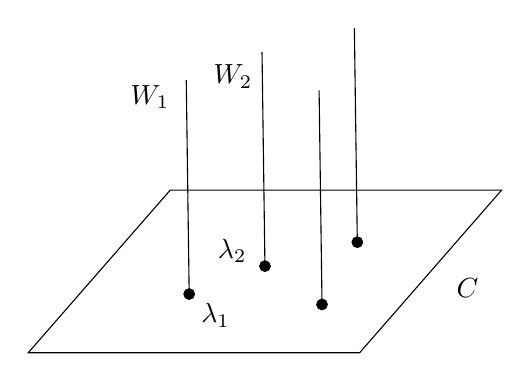
\begin{tikzpicture}[x=0.75pt,y=0.75pt,yscale=-1,xscale=1]
        %Shape: Parallelogram [id:dp548827135655336] 
        \draw   (129.38,106.55) -- (289.04,106.55) -- (220.61,184.94) -- (60.95,184.94) -- cycle ;
        %Shape: Circle [id:dp5536131887399003] 
        \draw  [color={rgb, 255:red, 0; green, 0; blue, 0 }  ,draw opacity=1 ][fill={rgb, 255:red, 0; green, 0; blue, 0 }  ,fill opacity=1 ] (135.95,156.64) .. controls (135.95,155.24) and (137.09,154.09) .. (138.5,154.09) .. controls (139.91,154.09) and (141.05,155.24) .. (141.05,156.64) .. controls (141.05,158.05) and (139.91,159.2) .. (138.5,159.2) .. controls (137.09,159.2) and (135.95,158.05) .. (135.95,156.64) -- cycle ;
        %Shape: Circle [id:dp3337454997914626] 
        \draw  [color={rgb, 255:red, 0; green, 0; blue, 0 }  ,draw opacity=1 ][fill={rgb, 255:red, 0; green, 0; blue, 0 }  ,fill opacity=1 ] (172.44,143.19) .. controls (172.44,141.78) and (173.59,140.64) .. (175,140.64) .. controls (176.4,140.64) and (177.55,141.78) .. (177.55,143.19) .. controls (177.55,144.6) and (176.4,145.74) .. (175,145.74) .. controls (173.59,145.74) and (172.44,144.6) .. (172.44,143.19) -- cycle ;
        %Shape: Circle [id:dp03436087376662322] 
        \draw  [color={rgb, 255:red, 0; green, 0; blue, 0 }  ,draw opacity=1 ][fill={rgb, 255:red, 0; green, 0; blue, 0 }  ,fill opacity=1 ] (199.95,161.64) .. controls (199.95,160.24) and (201.09,159.09) .. (202.5,159.09) .. controls (203.91,159.09) and (205.05,160.24) .. (205.05,161.64) .. controls (205.05,163.05) and (203.91,164.2) .. (202.5,164.2) .. controls (201.09,164.2) and (199.95,163.05) .. (199.95,161.64) -- cycle ;
        %Shape: Circle [id:dp09349939156591414] 
        \draw  [color={rgb, 255:red, 0; green, 0; blue, 0 }  ,draw opacity=1 ][fill={rgb, 255:red, 0; green, 0; blue, 0 }  ,fill opacity=1 ] (216.95,131.64) .. controls (216.95,130.24) and (218.09,129.09) .. (219.5,129.09) .. controls (220.91,129.09) and (222.05,130.24) .. (222.05,131.64) .. controls (222.05,133.05) and (220.91,134.2) .. (219.5,134.2) .. controls (218.09,134.2) and (216.95,133.05) .. (216.95,131.64) -- cycle ;
        %Straight Lines [id:da33322474104003263] 
        \draw    (137.09,53.57) -- (138.5,156.64) ;
        %Straight Lines [id:da7280355010137072] 
        \draw    (173.59,40.12) -- (175,143.19) ;
        %Straight Lines [id:da6839288750100709] 
        \draw    (201.09,58.57) -- (202.5,161.64) ;
        %Straight Lines [id:da9149673846486477] 
        \draw    (218.09,28.57) -- (219.5,131.64) ;
        
        % Text Node
        \draw (143.05,160.04) node [anchor=north west][inner sep=0.75pt]    {$\lambda _{1}$};
        % Text Node
        \draw (151.05,129.04) node [anchor=north west][inner sep=0.75pt]    {$\lambda _{2}$};
        % Text Node
        \draw (109.05,55.04) node [anchor=north west][inner sep=0.75pt]    {$W_{1}$};
        % Text Node
        \draw (149.05,45.04) node [anchor=north west][inner sep=0.75pt]    {$W_{2}$};
        % Text Node
        \draw (266.05,148.04) node [anchor=north west][inner sep=0.75pt]    {$\mathbb{C}$};
        
        
    \end{tikzpicture}
    \caption{The sheaf $\mathcal{F}_A \to \mathbb{C}$ of the linear operator $A: W \to W$. The support is the finite set $\text{Spec}(A) = \{\lambda_1, \dots, \lambda_m\}$. The stalk over $\lambda_i$ corresponds to the generalized eigenspace $W_i$.}
    \label{fig:figure5}
    \end{figure}
\begin{remark}
If $A$ is diagonalizable, $\mathcal{F}_A$ is a \textit{skyscraper sheaf}, supported only at the eigenvalues, with the stalk at $\lambda_i$ being the eigenspace $W_{\lambda_i}$. However, the decomposition \eqref{eq:4.8} depicted in Figure \ref{fig:figure5} does not determine the operator $A$ in general.

If there is a Jordan block of dimension $\alpha_i > 1$, the structure of the sheaf $\mathcal{F}_A$ in a formal (infinitesimal) neighborhood of the corresponding eigenvalue $\lambda_i$ encodes the nilpotent action $N = A - \lambda_i \text{id}_W$ on the generalized eigenspace $W_i$. This nilpotent structure, reflected in the flag \eqref{eq:4.6}, is captured by the non-trivial structure of the stalk $\mathcal{F}_{A,\lambda_i} \cong W_i$ as a module over the local ring $\mathcal{O}_{\C, \lambda_i}$ or its completion. The nilpotency is geometrically represented by this infinitesimal sheaf-theoretic behavior.
\end{remark}
\subsection{Projection-Valued Measures and Functional Calculus for Diagonalizable Operators}
\label{sec:pvm}

Henceforth in this section, we restrict our attention exclusively to linear operators $A: W \to W$ that are \textbf{diagonalizable} on a finite-dimensional complex vector space $W$. Recall that an operator $A$ is diagonalizable if and only if $W$ admits a basis consisting of eigenvectors of $A$, or equivalently, if its minimal polynomial has distinct roots. As we saw earlier, this is also equivalent to the geometric condition that the vector space $W$ decomposes as the direct sum of the eigenspaces of $A$. Let $\operatorname{Spec}(A) = \{\lambda_1, \dots, \lambda_m\} \subset \mathbb{C}$ denote the spectrum of $A$ (the set of distinct eigenvalues), and let $W_{\lambda_j} = \operatorname{Ker}(A - \lambda_j \operatorname{id}_W)$ be the eigenspace corresponding to the eigenvalue $\lambda_j$. By the definition of diagonalizability, the eigenspace decomposition provides an isomorphism:
\begin{equation*}
W \cong \bigoplus_{\lambda \in \operatorname{Spec}(A)} W_{\lambda}.
\end{equation*}
The action of the operator $A$ is completely determined by this decomposition and the associated eigenvalues: for any vector $w \in W$, if we decompose it uniquely as $w = \sum_{\lambda_j \in \operatorname{Spec}(A)} w_j$ with $w_j \in W_{\lambda_j}$, then $A(w) = \sum_{\lambda_j \in \operatorname{Spec}(A)} A(w_j) = \sum_{\lambda_j \in \operatorname{Spec}(A)} \lambda_j w_j$. Thus, $A$ simply acts as scalar multiplication by $\lambda_j$ on the subspace $W_{\lambda_j}$. This picture is captured by the interpretation of $A$ as the collection of its actions on the \dq{stalks} $W_\lambda$ over the discrete space $\operatorname{Spec}(A)$.

While intuitive, this description relies on the direct sum structure. We now develop an equivalent and powerful formalism that encodes such \dq{multiplication operators} purely in terms of projection operators associated with the eigenspaces. This projection-valued measure approach offers significant advantages, particularly for generalization.

\subsubsection{Projections, Orthogonal Projections, and Direct Sums}
\label{subsec:projections}

We begin by recalling and elaborating on the important properties of projection operators, which are the building blocks of spectral measures.

\begin{definition}[Projection Operator]
\label{def:projection_operator}
A linear operator $P: W \to W$ on a vector space $W$ is called a \textbf{projection} (or idempotent operator) if it satisfies the condition $P^2 = P$. The set of all projection operators on $W$ is denoted by $\operatorname{Proj}(W)$.
\end{definition}

Projections are linked to direct sum decompositions of the vector space.

\begin{proposition}[Projections and Direct Sums Correspondence]
\label{prop:proj_direct_sum}\,
\begin{enumerate}
    \item If $P \in \operatorname{Proj}(W)$, then $W$ decomposes as the direct sum of the image (range) and kernel (null space) of $P$:
        \begin{equation} \label{eq:4.12}
        W = \operatorname{Im}(P) \oplus \operatorname{Ker}(P).
        \end{equation}
        Furthermore, $P$ acts as the identity on $\operatorname{Im}(P)$ and as the zero operator on $\operatorname{Ker}(P)$. The operator $Q = \operatorname{id}_W - P$ is also a projection, called the complementary projection, satisfying $\operatorname{Im}(Q) = \operatorname{Ker}(P)$, $\operatorname{Ker}(Q) = \operatorname{Im}(P)$, and $PQ = QP = 0$.
    \item Conversely, given any direct sum decomposition $W = W'' \oplus W'$ into subspaces $W''$ and $W'$, there exists a unique projection operator $P: W \to W$ such that $\operatorname{Im}(P) = W''$ and $\operatorname{Ker}(P) = W'$. This operator is called the \textbf{projection onto $W''$ along $W'$}, and we denote it by $P''$. That is,
\begin{equation} \label{eq:4.13}
P'' : W \longrightarrow W, \quad \text{with } \operatorname{Im}(P'') = W'', \text{ and } \operatorname{Ker}(P'') = W'.
\end{equation}

\end{enumerate}
\end{proposition}
\begin{proof}\, 
    \begin{enumerate}
    \item For any $w \in W$, we can write
    \[
    w = Pw + (w - Pw).
    \]
    Clearly, $Pw \in \operatorname{Im}(P)$. Let $w' = w - Pw$. Then
    \[
    Pw' = P(w - Pw) = Pw - P^2w = Pw - Pw = 0,
    \]
    so $w' \in \operatorname{Ker}(P)$. This shows that
    \[
    W = \operatorname{Im}(P) + \operatorname{Ker}(P).
    \]
    To show the sum is direct, let $v \in \operatorname{Im}(P) \cap \operatorname{Ker}(P)$. Since $v \in \operatorname{Im}(P)$, there exists some $u \in W$ such that $v = Pu$. Since $v \in \operatorname{Ker}(P)$, we also have $Pv = 0$. Therefore,
    \[
    P^2u = 0,
    \]
    which implies $Pu = 0$, since $P^2 = P$. Hence, $v = 0$, proving the sum is direct.
    
    If $v \in \operatorname{Im}(P)$, then $v = Pu$, so $Pv = P^2u = Pu = v$. If $v \in \operatorname{Ker}(P)$, then $Pv = 0$.
    
    For $Q = \operatorname{id}_W - P$, we compute
    \[
    Q^2 = (\operatorname{id}_W - P)(\operatorname{id}_W - P) = \operatorname{id}_W - 2P + P^2 = \operatorname{id}_W - 2P + P = \operatorname{id}_W - P = Q.
    \]
    Thus, $Q^2 = Q$.
    
    Next, we find the kernel and image of $Q$:
    \[
    \operatorname{Ker}(Q) = \{w \mid (\operatorname{id}_W - P)w = 0\} = \{w \mid w = Pw\} = \operatorname{Im}(P),
    \]
    and
    \[
    \operatorname{Im}(Q) = \{(\operatorname{id}_W - P)w \mid w \in W\} = \operatorname{Ker}(P),
    \]
    as shown in the decomposition. Moreover, we have
    \[
    PQ = P(\operatorname{id}_W - P) = P - P^2 = 0,
    \]
    and
    \[
    QP = (\operatorname{id}_W - P)P = P - P^2 = 0.
    \]
    
    \item Given $W = W'' \oplus W'$, any $w \in W$ has a unique decomposition
    \[
    w = w'' + w',
    \]
    where $w'' \in W''$ and $w' \in W'$. Define $P(w) = w''$. This map is clearly linear. Its image is $W''$, and its kernel is
    \[
    \{w'' + w' \mid w'' = 0\} = W'.
    \]
    
    We now check idempotency:
    \[
    P^2(w) = P(w'') = w'' = P(w),
    \]
    since the decomposition of $w'' \in W''$ is $w'' = w'' + 0$.
    
    Uniqueness follows because any projection $P'$ with $\operatorname{Im}(P') = W''$ and $\operatorname{Ker}(P') = W'$ must map $w = w'' + w'$ to $P'(w'') + P'(w')$. Since $w'' \in \operatorname{Im}(P')$, we have $P'(w'') = w''$. Since $w' \in \operatorname{Ker}(P')$, we have $P'(w') = 0$. Thus,
    \[
    P'(w) = w'' = P(w).
    \]
\end{enumerate}
\end{proof}

When $W$ possesses an inner product structure $\langle \cdot, \cdot \rangle$, a special class of projections arises, characterized by compatibility with the inner product.

\begin{definition}[Orthogonal Projection]
\label{def:orthogonal_projection}
Let $(W, \langle \cdot, \cdot \rangle)$ be a finite-dimensional complex inner product space (i.e., a Hilbert space). A projection $P \in \operatorname{Proj}(W)$ is called an \textbf{orthogonal projection} if its image and kernel are orthogonal subspaces with respect to the inner product: $\operatorname{Im}(P) \perp \operatorname{Ker}(P)$. That is, $\langle Pw_1, (\operatorname{id}_W-P)w_2 \rangle = 0$ for all $w_1, w_2 \in W$.
\end{definition}

Orthogonal projections admit a important algebraic characterization involving the adjoint operator $P^*$, defined by $\langle Pw, v \rangle = \langle w, P^*v \rangle$ for all $v, w \in W$.

\begin{proposition}[Characterization of Orthogonal Projections]
\label{prop:orthog_proj_char}
A linear operator $P: W \to W$ on a finite-dimensional Hilbert space $W$ is an orthogonal projection if and only if it satisfies both $P^2 = P$ (idempotency) and $P^* = P$ (self-adjointness).
\end{proposition}
\begin{proof}
($\Rightarrow$) Assume that $P$ is an orthogonal projection. We already know that $P^2 = P$. We need to show that $P^* = P$. 

Since $W = \operatorname{Im}(P) \oplus \operatorname{Ker}(P)$ is an orthogonal decomposition, any $w, v \in W$ can be uniquely written as:
\[
w = w_1 + w_2 \quad \text{and} \quad v = v_1 + v_2,
\]
where $w_1, v_1 \in \operatorname{Im}(P)$ and $w_2, v_2 \in \operatorname{Ker}(P)$.

Therefore, we have:
\[
Pw = w_1 \quad \text{and} \quad Pv = v_1.
\]
We now compute the inner products:

\[
\langle Pw, v \rangle = \langle w_1, v_1 + v_2 \rangle = \langle w_1, v_1 \rangle + \langle w_1, v_2 \rangle = \langle w_1, v_1 \rangle,
\]
since $v_2 \in \operatorname{Ker}(P)$ and is orthogonal to $w_1 \in \operatorname{Im}(P)$.

Similarly:
\[
\langle w, Pv \rangle = \langle w_1 + w_2, v_1 \rangle = \langle w_1, v_1 \rangle + \langle w_2, v_1 \rangle = \langle w_1, v_1 \rangle,
\]
since $w_2 \in \operatorname{Ker}(P)$ and is orthogonal to $v_1 \in \operatorname{Im}(P)$.

Since we have:
\[
\langle Pw, v \rangle = \langle w, Pv \rangle \quad \text{for all} \quad w, v \in W,
\]
it follows that $P^* = P$.

($\Leftarrow$) Now assume that $P^2 = P$ and $P^* = P$. We know that $W = \operatorname{Im}(P) \oplus \operatorname{Ker}(P)$. Let $u \in \operatorname{Im}(P)$ and $v \in \operatorname{Ker}(P)$. We want to show that $\langle u, v \rangle = 0$.

Since $u \in \operatorname{Im}(P)$, we have $u = Pu$. Since $v \in \operatorname{Ker}(P)$, we have $Pv = 0$. Therefore:
\[
\langle u, v \rangle = \langle Pu, v \rangle = \langle u, P^*v \rangle \quad \text{(by the definition of adjoint)}.
\]
Since $P^* = P$, we obtain:
\[
\langle u, v \rangle = \langle u, Pv \rangle.
\]
Since $Pv = 0$, it follows that:
\[
\langle u, v \rangle = \langle u, 0 \rangle = 0.
\]
Thus, $\operatorname{Im}(P) \perp \operatorname{Ker}(P)$, and therefore, $P$ is an orthogonal projection.

\end{proof}

\subsubsection{Projection-Valued Measures (PVMs) for Diagonalizable Operators}
\label{subsec:pvm_def}

We now return to our setting of a diagonalizable operator $A: W \to W$ on a finite-dimensional complex vector space $W$, with the eigenspace decomposition $W = \bigoplus_{\lambda \in \operatorname{Spec}(A)} W_{\lambda}$. Let $\pi_{\lambda_j} \in \operatorname{Proj}(W)$ denote the unique projection onto the eigenspace $W_{\lambda_j}$ along the direct sum of the other eigenspaces $\bigoplus_{\lambda_k \neq \lambda_j} W_{\lambda_k}$. These individual projections satisfy important orthogonality relations.

\begin{lemma}[Properties of Eigenspace Projections]
\label{lemma:eig_proj_props}
Let $A$ be diagonalizable with distinct eigenvalues $\operatorname{Spec}(A) = \{\lambda_1, \dots, \lambda_m\}$, and let $\pi_{\lambda_j}$ be the projection onto $W_{\lambda_j}$ along $\bigoplus_{k \neq j} W_{\lambda_k}$. Then:
\begin{enumerate}
    \item $\sum_{j=1}^m \pi_{\lambda_j} = \operatorname{id}_W$ (Resolution of Identity).
    \item $\pi_{\lambda_j} \pi_{\lambda_k} = \delta_{jk} \pi_{\lambda_j}$ (Orthogonality of Projections).
\end{enumerate}
\end{lemma}
\begin{proof}\,

(1) Any $w \in W$ decomposes uniquely as $w = \sum_{k=1}^m w_k$ with $w_k \in W_{\lambda_k}$. By definition, $\pi_{\lambda_j}(w) = w_j$. Therefore, $(\sum_{j=1}^m \pi_{\lambda_j})(w) = \sum_{j=1}^m \pi_{\lambda_j}(w) = \sum_{j=1}^m w_j = w = \operatorname{id}_W(w)$. Since this holds for all $w$, $\sum \pi_{\lambda_j} = \operatorname{id}_W$.

(2) Consider $\pi_{\lambda_j} \pi_{\lambda_k}$. The image of $\pi_{\lambda_k}$ is $W_{\lambda_k}$. If $j \neq k$, then $W_{\lambda_k}$ is contained in the kernel of $\pi_{\lambda_j}$ (since $\operatorname{Ker}(\pi_{\lambda_j}) = \bigoplus_{l \neq j} W_{\lambda_l}$). Therefore, for $j \neq k$, $\pi_{\lambda_j} \pi_{\lambda_k} = 0$. If $j = k$, then $\pi_{\lambda_j} \pi_{\lambda_j} = (\pi_{\lambda_j})^2 = \pi_{\lambda_j}$ since $\pi_{\lambda_j}$ is a projection. Combining these, $\pi_{\lambda_j} \pi_{\lambda_k} = \delta_{jk} \pi_{\lambda_j}$.
\end{proof}

These projections allow us to define a set function whose values are operators, associating subsets of the complex plane to projections onto corresponding sums of eigenspaces.

\begin{definition}[Projection-Valued Measure (Finite-Dimensional Case)]
\label{def:pvm_finite}
Let $A: W \to W$ be a diagonalizable operator on a finite-dimensional complex vector space $W$. The \textbf{projection-valued measure (PVM)} or \textbf{spectral measure} associated with $A$ is the map
\begin{equation} \label{eq:4.14}
\pi_A : \mathcal{P}(\mathbb{C}) \longrightarrow \operatorname{Proj}(W)
\end{equation}
(where $\mathcal{P}(\mathbb{C})$ is the power set of $\mathbb{C}$) defined by assigning to each subset $E \subseteq \mathbb{C}$ the projection onto the sum of eigenspaces corresponding to eigenvalues lying within $E$:
\[ E \mapsto \pi_A(E) \coloneqq \sum_{\lambda_j \in E \cap \operatorname{Spec}(A)} \pi_{\lambda_j} \]
where $\pi_{\lambda_j}$ is the projection onto the eigenspace $W_{\lambda_j}$ along $\bigoplus_{k \neq j} W_{\lambda_k}$. If $E \cap \operatorname{Spec}(A)$ is empty, the sum is empty and defined as the zero operator.
\end{definition}

\begin{remark}[Dependence on Spectrum]
Observe that although the domain is formally written as $\mathcal{P}(\mathbb{C})$, the map $\pi_A$ is constant on sets $E$ having the same intersection with the finite set $\operatorname{Spec}(A)$. It is non-zero only for sets $E$ that contain at least one eigenvalue of $A$. Effectively, $\pi_A$ is supported on $\operatorname{Spec}(A)$.
\end{remark}

\begin{remark}[Orthogonality for Normal Operators]
\label{rem:pvm_normal}
If $W$ is equipped with an inner product $\langle \cdot, \cdot \rangle$ and the operator $A$ is \textbf{normal} (i.e., $A$ commutes with its adjoint, $AA^* = A^*A$), then $A$ is diagonalizable, and its eigenspaces corresponding to distinct eigenvalues are mutually orthogonal: $W_{\lambda_j} \perp W_{\lambda_k}$ for $j \neq k$. In this case, the direct sum $W = \bigoplus_{\lambda_j \in \operatorname{Spec}(A)} W_{\lambda_j}$ is an orthogonal direct sum. Consequently, each individual projection $\pi_{\lambda_j}$ is an orthogonal projection ($\pi_{\lambda_j}^* = \pi_{\lambda_j}$), and the PVM $\pi_A(E) = \sum_{\lambda_j \in E \cap \operatorname{Spec}(A)} \pi_{\lambda_j}$ is also an orthogonal projection for every $E \subseteq \mathbb{C}$. This holds, in particular, if $A$ is self-adjoint ($A^*=A$) or unitary ($A^*A = AA^* = \operatorname{id}_W$).
\end{remark}

The map $\pi_A$ exhibits properties strongly analogous to those of a classical (scalar-valued) measure, justifying its name.

\begin{proposition}[Properties of the PVM $\pi_A$]
\label{prop:pvm_props}
The map $\pi_A: \mathcal{P}(\mathbb{C}) \to \operatorname{Proj}(W)$ defined above satisfies the following properties:
\begin{itemize}
    \item[(i)] \textbf{Null Empty Set:} $\pi_A(\emptyset) = 0$.
    \item[(ii)] \textbf{Normalization:} $\pi_A(\mathbb{C}) = \pi_A(\operatorname{Spec}(A)) = \operatorname{id}_W$.
    \item[(iii)] \textbf{Finite Additivity:} If $E_1, E_2 \subseteq \mathbb{C}$ are disjoint subsets, then
        \[ \pi_A(E_1 \cup E_2) = \pi_A(E_1) + \pi_A(E_2). \]
        More generally, for pairwise disjoint $E_1, \dots, E_n$, $\pi_A(\cup_{i=1}^n E_i) = \sum_{i=1}^n \pi_A(E_i)$.
    \item[(iv)] \textbf{Multiplicativity/Intersection Property:} For any $E_1, E_2 \subseteq \mathbb{C}$,
        \[ \pi_A(E_1 \cap E_2) = \pi_A(E_1) \pi_A(E_2). \]
\end{itemize}
These properties imply, in particular, that projections associated with disjoint sets commute and their product is zero: if $E_1 \cap E_2 = \emptyset$, then $\pi_A(E_1) \pi_A(E_2) = \pi_A(E_1 \cap E_2) = \pi_A(\emptyset) = 0$.
\end{proposition}
\begin{proof}
Let $S = \operatorname{Spec}(A)$.

(i) $\pi_A(\emptyset) = \sum_{\lambda \in \emptyset \cap S} \pi_\lambda = 0$ (sum over empty set).

(ii) $\pi_A(\mathbb{C}) = \sum_{\lambda \in \mathbb{C} \cap S} \pi_\lambda = \sum_{\lambda \in S} \pi_\lambda = \operatorname{id}_W$ by Lemma \ref{lemma:eig_proj_props}(1). Similarly for $\pi_A(S)$.

(iii) If $E_1 \cap E_2 = \emptyset$, then $E_1 \cap S$ and $E_2 \cap S$ are disjoint subsets of $S$. The set of eigenvalues in the union is the disjoint union of the eigenvalues in each set: $(E_1 \cup E_2) \cap S = (E_1 \cap S) \cup (E_2 \cap S)$. Therefore,
    \[ \pi_A(E_1 \cup E_2) = \sum_{\lambda \in (E_1 \cup E_2) \cap S} \pi_\lambda = \sum_{\lambda \in (E_1 \cap S)} \pi_\lambda + \sum_{\lambda \in (E_2 \cap S)} \pi_\lambda = \pi_A(E_1) + \pi_A(E_2). \]

(iv) Using the definition and the orthogonality property $\pi_\lambda \pi_\mu = \delta_{\lambda\mu} \pi_\lambda$ from Lemma \ref{lemma:eig_proj_props}(2):
\begin{align*} \pi_A(E_1) \pi_A(E_2) &= \left( \sum_{\lambda \in E_1 \cap S} \pi_\lambda \right) \left( \sum_{\mu \in E_2 \cap S} \pi_\mu \right) \\ &= \sum_{\lambda \in E_1 \cap S} \sum_{\mu \in E_2 \cap S} \pi_\lambda \pi_\mu \\ &= \sum_{\lambda \in E_1 \cap S} \sum_{\mu \in E_2 \cap S} \delta_{\lambda\mu} \pi_\lambda \\ &= \sum_{\lambda \in (E_1 \cap S) \cap (E_2 \cap S)} \pi_\lambda \quad (\text{only terms with } \lambda=\mu \text{ survive}) \\ &= \sum_{\lambda \in (E_1 \cap E_2) \cap S} \pi_\lambda \\ &= \pi_A(E_1 \cap E_2). \qedhere \end{align*}
\end{proof}

The set of projections $\{\pi_{\lambda_j}\}_{\lambda_j \in \operatorname{Spec}(A)}$ associated with individual eigenvalues forms the core of the PVM. They constitute a complete set of mutually orthogonal (in the sense $\pi_j \pi_k = 0$ for $j \neq k$) projections summing to the identity, often called a \textbf{resolution of the identity} associated with $A$.

\subsubsection{Connection to Probability Measures}

The designation of the map $\pi_A : \mathcal{P}(\mathbb{C}) \longrightarrow \operatorname{Proj}(W)$ as a projection valued measure invites a comparison to the more familiar concept of classical, scalar-valued measures, particularly probability measures. While PVMs are operator-valued, their mathematical properties enable the construction of classical probability measures associated with vectors in the underlying space, thereby providing a general framework.

We first recall the basics of classical measure theory and probability spaces.

\begin{definition}[Measurable Space and $\sigma$-Algebra]
A \textbf{measurable space} is a pair $(X, \Sigma)$, where $X$ is a non-empty set, often called the \dq{sample space} or \dq{universe of outcomes,} and $\Sigma$ is a \textbf{$\sigma$-algebra} (or $\sigma$-field) of subsets of $X$. $\Sigma$ is a collection of subsets of $X$ satisfying:
\begin{enumerate}
    \item $X \in \Sigma$ (the entire space is measurable).
    \item If $E \in \Sigma$, then its complement $X \setminus E$ is also in $\Sigma$ (closure under complementation).
    \item If $\{E_i\}_{i=1}^\infty$ is a countable collection of sets in $\Sigma$, then their union $\cup_{i=1}^\infty E_i$ is in $\Sigma$ (closure under countable unions).
\end{enumerate}
The elements of $\Sigma$ are called \dq{measurable sets} or, in probabilistic contexts, \dq{events.}
\end{definition}

\begin{definition}[Positive Measure]
A \textbf{positive measure} on a measurable space $(X, \Sigma)$ is a function $\mu: \Sigma \to [0, \infty]$ (the set of non-negative extended real numbers) such that:
\begin{enumerate}
    \item $\mu(\emptyset) = 0$ (the measure of the empty set is zero).
    \item (Countable Additivity / $\sigma$-additivity) For any countable sequence $\{E_i\}_{i=1}^\infty$ of pairwise disjoint sets in $\Sigma$ (i.e., $E_i \cap E_j = \emptyset$ for $i \neq j$),
        \[ \mu\left(\bigcup_{i=1}^\infty E_i\right) = \sum_{i=1}^\infty \mu(E_i). \]
\end{enumerate}
\end{definition}
From these axioms, several standard properties of measures follow, including:
\begin{itemize}
    \item Finite Additivity: For any finite collection of pairwise disjoint sets $E_1, \dots, E_n \in \Sigma$, $\mu(\cup_{k=1}^n E_k) = \sum_{k=1}^n \mu(E_k)$.
    \item Monotonicity: If $E, F \in \Sigma$ and $E \subseteq F$, then $\mu(E) \le \mu(F)$.
    \item Subadditivity: For any countable collection $\{E_i\}_{i=1}^\infty$ of sets in $\Sigma$ (not necessarily disjoint), $\mu(\cup_{i=1}^\infty E_i) \le \sum_{i=1}^\infty \mu(E_i)$.
    \item Continuity from below: If $E_1 \subseteq E_2 \subseteq \dots$ is an increasing sequence of sets in $\Sigma$ and $E = \cup_{n=1}^\infty E_n$, then $\mu(E) = \lim_{n\to\infty} \mu(E_n)$.
    \item Continuity from above: If $E_1 \supseteq E_2 \supseteq \dots$ is a decreasing sequence of sets in $\Sigma$, $E = \cap_{n=1}^\infty E_n$, and $\mu(E_1) < \infty$, then $\mu(E) = \lim_{n\to\infty} \mu(E_n)$.
\end{itemize}

\begin{definition}[Finite Measures and Probability Measures]\,
\begin{enumerate}
    \item A positive measure $\mu$ is \textbf{finite} if $\mu(X) < \infty$.
    \item A positive measure $P$ on $(X, \Sigma)$ is a \textbf{probability measure} if $P(X) = 1$. The triple $(X, \Sigma, P)$ is then termed a \textbf{probability space}.
\end{enumerate}
More generally, one defines signed measures (real-valued) and complex measures, both satisfying countable additivity.
\end{definition}
In the context of a PVM $\pi_A$ for a diagonalizable operator $A$ on a finite-dimensional space $W$, the spectrum $\operatorname{Spec}(A)$ is a finite set. We can take $X = \operatorname{Spec}(A)$ and $\Sigma = \mathcal{P}(\operatorname{Spec}(A))$ (the power set of the spectrum). In this scenario, any finitely additive set function automatically satisfies countable additivity because any countable disjoint union can only contain finitely many non-empty sets.

The PVM $\pi_A$, as defined in Definition \ref{def:pvm_finite} has many parallels to the axiomatic structure of a probability measure, especially concerning its behavior under set operations (Proposition \ref{prop:pvm_props}).

\begin{itemize}
    \item[(i)] \textbf{Null Empty Set: $\pi_A(\emptyset) = 0$.}
    This is structurally identical to $P(\emptyset)=0$. The PVM assigns the zero operator to the empty set of spectral values, signifying that the \dq{spectral content} associated with no eigenvalues is trivial (projection onto the zero-dimensional subspace $\{0_W\}$).

    \item[(ii)] \textbf{Normalization / Total Measure: $\pi_A(\mathbb{C}) = \pi_A(\operatorname{Spec}(A)) = \operatorname{id}_W$.}
    This parallels $P(X)=1$. The identity operator $\operatorname{id}_W$ serves as the operatorial analogue of \dq{total probability} or \dq{certainty.} It confirms that the entire space $W$ is accounted for by the spectral decomposition $W = \bigoplus_{\lambda \in \operatorname{Spec}(A)} W_{\lambda}$. The sum of projections onto all distinct eigenspaces, $\sum_{\lambda \in \operatorname{Spec}(A)} \pi_\lambda = \operatorname{id}_W$ (see Lemma \ref{lemma:eig_proj_props}).

    \item[(iii)] \textbf{Finite Additivity: $\pi_A(E_1 \cup E_2) = \pi_A(E_1) + \pi_A(E_2)$ for disjoint $E_1, E_2 \subseteq \mathbb{C}$.}
    This mirrors the additivity $P(E_1 \cup E_2) = P(E_1) + P(E_2)$ for mutually exclusive events. The PVM property follows from its definition as a sum over individual eigenspace projections:
    \[ \pi_A(E_1 \cup E_2) = \sum_{\lambda \in (E_1 \cap S) \cup (E_2 \cap S)} \pi_\lambda = \sum_{\lambda \in E_1 \cap S} \pi_\lambda + \sum_{\lambda \in E_2 \cap S} \pi_\lambda = \pi_A(E_1) + \pi_A(E_2), \]
    where $S = \operatorname{Spec}(A)$ and the disjointness of $E_1, E_2$ implies disjointness of $E_1 \cap S$ and $E_2 \cap S$. The sum is one of linear operators. For this sum $\pi_A(E_1) + \pi_A(E_2)$ to itself be a projection (which $\pi_A(E_1 \cup E_2)$ is), a necessary and sufficient condition is that $\pi_A(E_1)\pi_A(E_2) = 0$ and $\pi_A(E_2)\pi_A(E_1) = 0$. This condition is indeed satisfied due to property (iv) below, as $E_1 \cap E_2 = \emptyset \implies \pi_A(E_1)\pi_A(E_2) = \pi_A(\emptyset) = 0$. The image of $\pi_A(E_1 \cup E_2)$ is then the direct sum of the images of $\pi_A(E_1)$ and $\pi_A(E_2)$.
\end{itemize}

The major difference from classical probability measures is that $\pi_A(E)$ is an operator (a projection) and not a scalar value in $[0,1]$. However, this operator-valued structure provides a way to generate classical scalar measures, including probability measures, when an inner product and specific vectors (states) are introduced. This is particularly transparent for normal operators, where the PVM consists of orthogonal projections.

Let $W$ be a finite-dimensional complex inner product space, and let $A$ be a normal operator on $W$. Then its PVM $\pi_A(E)$ consists of orthogonal projections (i.e., $\pi_A(E)^* = \pi_A(E)$ and $\pi_A(E)^2 = \pi_A(E)$). For any vector $\psi \in W$, consider the map $\mu_\psi: \mathcal{P}(\operatorname{Spec}(A)) \to [0, \infty)$ defined by:
\[ \mu_\psi(E) \coloneqq \langle \psi, \pi_A(E)\psi \rangle. \]
Since $\pi_A(E)$ is an orthogonal projection, 
\begin{align*}
    \langle \psi, \pi_A(E)\psi \rangle &= \langle \psi, \pi_A(E)^*\pi_A(E)\psi \rangle \\ 
    &= \langle \pi_A(E)\psi, \pi_A(E)\psi \rangle \\ 
    &= \|\pi_A(E)\psi\|^2 \ge 0.
\end{align*}
This map $\mu_\psi$ is a finite positive measure on $\operatorname{Spec}(A)$:
\begin{enumerate}
    \item $\mu_\psi(\emptyset) = \|\pi_A(\emptyset)\psi\|^2 = \|0\psi\|^2 = 0$.
    \item (Finite Additivity) For disjoint $E_1, E_2 \subseteq \operatorname{Spec}(A)$:
    The projections $\pi_A(E_1)$ and $\pi_A(E_2)$ are orthogonal and their images are orthogonal subspaces because $E_1 \cap E_2 = \emptyset \implies \pi_A(E_1)\pi_A(E_2)=0$. This means that $\pi_A(E_1)\psi$ is orthogonal to $\pi_A(E_2)\psi$.
    Thus,
    \begin{align*} \mu_\psi(E_1 \cup E_2) &= \|\pi_A(E_1 \cup E_2)\psi\|^2 = \|(\pi_A(E_1) + \pi_A(E_2))\psi\|^2 \\ &= \|\pi_A(E_1)\psi + \pi_A(E_2)\psi\|^2 \\ &= \|\pi_A(E_1)\psi\|^2 + \|\pi_A(E_2)\psi\|^2 \quad (\text{by the Pythagorean theorem}) \\ &= \mu_\psi(E_1) + \mu_\psi(E_2). \end{align*}
\end{enumerate}
The total measure is $\mu_\psi(\operatorname{Spec}(A)) = \|\pi_A(\operatorname{Spec}(A))\psi\|^2 = \|\operatorname{id}_W \psi\|^2 = \|\psi\|^2$.
Crucially, if the vector $\psi$ is normalized such that $\|\psi\|=1$, then $\mu_\psi(\operatorname{Spec}(A)) = 1$. In this case, $\mu_\psi$ becomes a classical \textbf{probability measure} on the finite set $\operatorname{Spec}(A)$. Thus, the PVM $\pi_A$, while operator-valued, naturally induces a family of probability measures, parameterized by the choice of a normalized vector $\psi$. Each such $\mu_\psi$ describes a probability distribution over the possible spectral values of $A$.

More generally, for any pair of vectors $\phi, \psi \in W$, the function $\mu_{\phi,\psi}(E) \coloneqq \langle \phi, \pi_A(E)\psi \rangle$ defines a complex measure on $\operatorname{Spec}(A)$. These are essential for defining the integral $\langle \phi, f(A)\psi \rangle = \int f(\lambda)d\mu_{\phi,\psi}(\lambda)$ for complex-valued functions $f$.

Once we have the probability measure $\mu_\psi$ associated with a normalized vector $\psi$ and a self-adjoint operator $A$ (whose spectrum is real), we can define the expectation of a function $f: \operatorname{Spec}(A) \to \mathbb{R}$ in the classical sense:
\[ \mathbb{E}_{\mu_\psi}[f] \coloneqq \int_{\operatorname{Spec}(A)} f(\lambda) \, d\mu_\psi(\lambda) = \sum_{\lambda_j \in \operatorname{Spec}(A)} f(\lambda_j) \mu_\psi(\{\lambda_j\}). \]
Using the functional calculus $f(A) = \sum_{\lambda_j \in \operatorname{Spec}(A)} f(\lambda_j) \pi_{\lambda_j}$ and $\mu_\psi(\{\lambda_j\}) = \langle \psi, \pi_{\lambda_j}\psi \rangle = \|\pi_{\lambda_j}\psi\|^2$, we find:
\begin{align*} \langle \psi, f(A)\psi \rangle &= \left\langle \psi, \sum_{\lambda_j \in \operatorname{Spec}(A)} f(\lambda_j) \pi_{\lambda_j} \psi \right\rangle \\ &= \sum_{\lambda_j \in \operatorname{Spec}(A)} f(\lambda_j) \langle \psi, \pi_{\lambda_j} \psi \rangle \\ &= \sum_{\lambda_j \in \operatorname{Spec}(A)} f(\lambda_j) \mu_\psi(\{\lambda_j\}) \\ &= \mathbb{E}_{\mu_\psi}[f]. \end{align*}
In particular, for $f(\lambda) = \lambda$, the \dq{average value} $\langle \psi, A\psi \rangle$ is precisely the expectation $\mathbb{E}_{\mu_\psi}[\lambda]$, where $\lambda$ is viewed as a random variable distributed according to $\mu_\psi$. Similarly, the variance can be defined:
\[ \operatorname{Var}_{\mu_\psi}(\lambda) = \mathbb{E}_{\mu_\psi}[(\lambda - \mathbb{E}_{\mu_\psi}[\lambda])^2] = \langle \psi, (A - \langle \psi, A\psi \rangle \operatorname{id}_W)^2 \psi \rangle. \]
This shows how the operatorial PVM framework connects directly to classical statistical concepts through the vector-dependent probability measures.

The PVM property (iv) $\pi_A(E_1 \cap E_2) = \pi_A(E_1) \pi_A(E_2)$ is another major difference from the properties of typical probability measures. For probabilities, $P(E_1 \cap E_2) = P(E_1)P(E_2)$ holds if and only if the events $E_1$ and $E_2$ are \textbf{statistically independent}. Independence is a specific relationship between events contingent on a particular probability measure $P$, not an axiom of probability measures themselves.

In contrast, for a PVM $\pi_A$ derived from a single operator $A$, the multiplicative property $\pi_A(E_1 \cap E_2) = \pi_A(E_1)\pi_A(E_2)$ is an inherent structural property. It follows from the idempotency and mutual orthogonality of the elementary spectral projections $\pi_\lambda \pi_\mu = \delta_{\lambda\mu}\pi_\lambda$. Since all $\pi_A(E)$ are sums of these $\pi_\lambda$, they all commute: $\pi_A(E_1)\pi_A(E_2) = \pi_A(E_2)\pi_A(E_1)$. This commutativity of projection values for any two sets is a key feature. The property reflects the underlying logic of spectral decomposition: applying a \dq{filter} for eigenvalues in $E_2$ and then a \dq{filter} for eigenvalues in $E_1$ is equivalent to applying a single \dq{filter} for eigenvalues in $E_1 \cap E_2$. This robust algebraic property is essential for ensuring that the functional calculus $f \mapsto f(A)$ defines an algebra homomorphism (specifically, $(fg)(A)=f(A)g(A)$).

The true power of this measure-theoretic perspective, especially its connection to probability, becomes fully apparent in the context of infinite-dimensional Hilbert spaces and operators with continuous spectra (as discussed in Section \ref{sec:hilbert}).
\begin{enumerate}
    \item The PVM $\pi_A$ associated with a self-adjoint operator $A$ is defined on the Borel $\sigma$-algebra $\mathcal{B}(\sigma(A))$ of its spectrum.
    \item The crucial property is \textbf{countable additivity (strong operator topology-convergence)}: for any sequence $\{E_i\}_{i=1}^\infty$ of pairwise disjoint Borel sets,
        \[ \pi_A\left(\bigcup_{i=1}^\infty E_i\right)\psi = \sum_{i=1}^\infty \pi_A(E_i)\psi \quad (\text{for all } \psi \in \mathcal{H}). \]
\end{enumerate}
This SOT-countable additivity of the PVM $\pi_A$ is precisely the condition required to ensure that each derived scalar function $\mu_\psi(E) = \|\pi_A(E)\psi\|^2$ is a true, countably additive probability measure on $(\sigma(A), \mathcal{B}(\sigma(A)))$ when $\|\psi\|=1$. This mathematical structure supports the probabilistic interpretation of quantum measurements, even for observables with continuous spectra like position or momentum, where sums turn into integrals against probability measures determined by the quantum state.

To summarize, while PVMs are fundamentally operator-valued, they share core axiomatic traits with scalar measures, particularly concerning normalization and additivity for disjoint sets. For normal operators on an inner product space, the PVM, being composed of orthogonal projections, naturally allows the construction of a family of classical positive scalar measures $\mu_\psi(E) = \|\pi_A(E)\psi\|^2$. When the vector $\psi$ is normalized, $\mu_\psi$ becomes a probability measure on the spectrum of $A$. This provides a purely mathematical pathway to probabilistic interpretations. The expectation values formed with respect to these probability measures align perfectly with the inner product expressions like $\langle \psi, f(A)\psi \rangle$. The distinctive multiplicative property of PVMs, $\pi_A(E_1 \cap E_2) = \pi_A(E_1)\pi_A(E_2)$, is an algebraic feature that has no direct counterpart in general probability theory beyond the special case of statistical independence; for PVMs, it is important for the homomorphism property of the functional calculus. Overall, PVMs offer a mathematical framework in which operator-valued measures can produce classical probability distributions when applied to specific states.

\subsubsection{The Functional Calculus for Diagonalizable Operators}
\label{subsec:functional_calculus_finite}

The primary purpose of the PVM formalism is to provide a unified way to define functions of the operator $A$. This is known as the functional calculus. Applying functions to operators naturally arises in various contexts, such as solving systems of linear differential equations ($e^{tA}$), defining norms or condition numbers of matrices, and formulating observables and their evolution in quantum mechanics.

First, the operator $A$ itself can be reconstructed from its eigenvalues and the corresponding projections. Since $A$ acts as $\lambda_j \operatorname{id}_{W_{\lambda_j}}$ on the image of $\pi_{\lambda_j}$, and $\sum \pi_{\lambda_j} = \operatorname{id}_W$, we can write $A$ as a linear combination of these projections, weighted by the eigenvalues.

\begin{proposition}[Spectral Decomposition of A]
\label{prop:spectral_decomp}
Let $A$ be a diagonalizable operator with distinct eigenvalues $\operatorname{Spec}(A) = \{\lambda_1, \dots, \lambda_m\}$ and corresponding eigenspace projections $\pi_{\lambda_j}$. Then $A$ can be expressed as:
\begin{equation} \label{eq:4.15}
A = \sum_{j=1}^m \lambda_j \pi_{\lambda_j}.
\end{equation}
This is often written suggestively as an integral with respect to the PVM:
\[ A = \int_{\mathbb{C}} \lambda \, d\pi_A(\lambda) \quad \text{or} \quad A = \int_{\operatorname{Spec}(A)} \lambda \, d\pi_A(\lambda). \]
\end{proposition}
\begin{proof}
    Let $w \in W$. Decompose $w = \sum_{k=1}^m w_k$ where 
    \[
    w_k = \pi_{\lambda_k}(w) \in W_{\lambda_k}.
    \]
    Then 
    \[
    A(w) = \sum_{k=1}^m A(w_k) = \sum_{k=1}^m \lambda_k w_k.
    \]
    Now compute the action of the sum:
    \[
    \left( \sum_{j=1}^m \lambda_j \pi_{\lambda_j} \right)(w) = \sum_{j=1}^m \lambda_j \pi_{\lambda_j} \left( \sum_{k=1}^m w_k \right) = \sum_{j=1}^m \sum_{k=1}^m \lambda_j \pi_{\lambda_j} w_k.
    \]
    Since $w_k \in W_{\lambda_k}$, we have
    \[
    \pi_{\lambda_j} w_k = \delta_{jk} w_k.
    \]
    Thus, the sum becomes
    \[
    \sum_{j=1}^m \sum_{k=1}^m \lambda_j \delta_{jk} w_k = \sum_{k=1}^m \lambda_k w_k.
    \]
    This equals $A(w)$. Since the operators agree on all $w$, they are equal. The integral notation emphasizes that $A$ is synthesized from its spectral values $\lambda$ weighted by the spectral measure $\pi_A$ concentrated at those values.
    
\end{proof}

This spectral decomposition naturally suggests how to define $f(A)$ for functions $f$. If $p(z) = \sum_{k=0}^N c_k z^k$ is a polynomial, then using $A^k = (\sum \lambda_j \pi_{\lambda_j})^k = \sum \lambda_j^k \pi_{\lambda_j}$ (due to $\pi_j \pi_l = \delta_{jl} \pi_j$), we find
\[ p(A) = \sum_{k=0}^N c_k A^k = \sum_{k=0}^N c_k \left( \sum_{j=1}^m \lambda_j^k \pi_{\lambda_j} \right) = \sum_{j=1}^m \left( \sum_{k=0}^N c_k \lambda_j^k \right) \pi_{\lambda_j} = \sum_{j=1}^m p(\lambda_j) \pi_{\lambda_j}. \]
This calculation shows that applying a polynomial $p$ to the operator $A$ is equivalent to applying $p$ to each eigenvalue $\lambda_j$ and summing the results weighted by the corresponding projection $\pi_{\lambda_j}$. This motivates extending the definition from polynomials to arbitrary functions defined on the spectrum of $A$.

\begin{definition}[Functional Calculus]
\label{def:functional_calculus}
Let $A: W \to W$ be a diagonalizable operator with spectral measure $\pi_A$. Let $f: \operatorname{Spec}(A) \to \mathbb{C}$ be any function defined on the spectrum of $A$. (We can extend $f$ to all of $\mathbb{C}$ arbitrarily, e.g., by setting $f(\lambda)=0$ for $\lambda \notin \operatorname{Spec}(A)$, as only its values on $\operatorname{Spec}(A)$ affect the sum). The operator $f(A): W \to W$ is defined as:
\begin{equation} \label{eq:4.16}
f(A) \coloneqq \sum_{\lambda_j \in \operatorname{Spec}(A)} f(\lambda_j) \pi_{\lambda_j}.
\end{equation}
This can also be written using the integral notation:
\[ f(A) = \int_{\operatorname{Spec}(A)} f(\lambda) \, d\pi_A(\lambda). \]
This map $f \mapsto f(A)$ is called the \textbf{functional calculus} for the diagonalizable operator $A$.
\end{definition}

This definition provides a consistent and computationally effective way to apply functions to operators.
\begin{example}[Applying Functions to Functional Calculus]\,
\begin{itemize}
    \item The operator exponential $e^{tA}$ (important for solving linear ODE systems $\dot{x}=Ax$) is given by 
    \[e^{tA} = \sum_{j=1}^m e^{t\lambda_j} \pi_{\lambda_j}.\]
    \item If $0 \notin \operatorname{Spec}(A)$, meaning $A$ is invertible, we can define $f(\lambda) = 1/\lambda$ for $\lambda \in \operatorname{Spec}(A)$. Then the inverse is 
    \[A^{-1} = f(A) = \sum_{j=1}^m \frac{1}{\lambda_j} \pi_{\lambda_j}.\] 
    We can verify this: 
    \[A A^{-1} = (\sum_{k=1}^m \lambda_k \pi_{\lambda_k})(\sum_{j=1}^m \frac{1}{\lambda_j} \pi_{\lambda_j}) = \sum_{j,k=1}^m \frac{\lambda_k}{\lambda_j} \pi_{\lambda_k} \pi_{\lambda_j} = \sum_{j=1}^m \frac{\lambda_j}{\lambda_j} \pi_{\lambda_j} = \sum_{j=1}^m \pi_{\lambda_j} = \operatorname{id}_W.\]
    \item Consider the matrix $A = \begin{pmatrix} 2 & 0 \\ 0 & -1 \end{pmatrix}$. The spectrum of $A$ is given by 
    \[
    \operatorname{Spec}(A) = \{2, -1\}.
    \]
    Let 
    \[
    W_2 = \operatorname{span}\left\{ \begin{pmatrix} 1 \\ 0 \end{pmatrix} \right\}, \quad W_{-1} = \operatorname{span}\left\{ \begin{pmatrix} 0 \\ 1 \end{pmatrix} \right\}.
    \]
    The corresponding projection operators are
    \[
    \pi_2 = \begin{pmatrix} 1 & 0 \\ 0 & 0 \end{pmatrix}, \quad \pi_{-1} = \begin{pmatrix} 0 & 0 \\ 0 & 1 \end{pmatrix}.
    \]
    
    Now, let $f(x) = x^3$. We can compute $f(A)$ as follows:
    \[
    f(A) = f(2)\pi_2 + f(-1)\pi_{-1} = 8\pi_2 + (-1)\pi_{-1} = \begin{pmatrix} 8 & 0 \\ 0 & -1 \end{pmatrix},
    \]
    which is equal to $A^3$.
    
    Next, let $g(x) = \sqrt{x}$ (defined for positive eigenvalues). If 
    \[
    A = \begin{pmatrix} 4 & 0 \\ 0 & 9 \end{pmatrix},
    \]
    then we compute $g(A)$ as follows:
    \[
    g(A) = \sqrt{4}\pi_4 + \sqrt{9}\pi_9 = 2\pi_4 + 3\pi_9 = \begin{pmatrix} 2 & 0 \\ 0 & 3 \end{pmatrix},
    \]
    which is one possible square root of $A$.
\end{itemize}
\end{example}

The functional calculus possesses important algebraic properties, formalizing the idea that calculations with $f(A)$ mirror calculations with the function $f$ itself on the spectrum. Let $\mathcal{F}(\operatorname{Spec}(A))$ be the algebra of complex-valued functions on the finite set $\operatorname{Spec}(A)$ equipped with pointwise addition, scalar multiplication, and pointwise multiplication. Let $\mathcal{L}(W)$ be the algebra of linear operators on $W$.

\begin{theorem}[Properties of the Functional Calculus]
\label{thm:func_calc_props}
The functional calculus map $\Psi: \mathcal{F}(\operatorname{Spec}(A)) \to \mathcal{L}(W)$ defined by $\Psi(f) = f(A)$ is an algebra homomorphism. That is, for $f, g \in \mathcal{F}(\operatorname{Spec}(A))$ and $c \in \mathbb{C}$:
\begin{enumerate}
    \item $\Psi(f+g) = (f+g)(A) = f(A) + g(A) = \Psi(f) + \Psi(g)$ (Additivity).
    \item $\Psi(cf) = (cf)(A) = c f(A) = c \Psi(f)$ (Homogeneity).
    \item $\Psi(fg) = (fg)(A) = f(A) g(A) = \Psi(f) \Psi(g)$ (Multiplicativity).
    \item $\Psi(\mathbf{1}) = \mathbf{1}(A) = \operatorname{id}_W$, where $\mathbf{1}$ is the constant function $f(\lambda)=1$.
    \item $\Psi(\mathrm{id}_{\mathbb{C}}) = \mathrm{id}_{\mathbb{C}}(A) = A$, where $\mathrm{id}_{\mathbb{C}}$ is the identity function $f(\lambda)=\lambda$.
\end{enumerate}
If $W$ is equipped with an inner product and $A$ is a normal operator, then $\Psi$ is furthermore a *-homomorphism, meaning it respects the adjoint operation (involution):
\begin{enumerate}
    \item[6.] $\Psi(\bar{f}) = \bar{f}(A) = (f(A))^* = (\Psi(f))^*$, where $\bar{f}$ is the complex conjugate function $\bar{f}(\lambda) = \overline{f(\lambda)}$.
\end{enumerate}
\end{theorem}
\begin{proof}
Properties (1) and (2) follow directly from the linearity of the summation in the definition \eqref{eq:4.16}:
\begin{align*}
    (f+g)(A) &= \sum (f+g)(\lambda_j) \pi_j\\ 
    &= \sum (f(\lambda_j)+g(\lambda_j)) \pi_j \\ 
    &= \sum f(\lambda_j)\pi_j + \sum g(\lambda_j)\pi_j \\ 
    &= f(A)+g(A)
\end{align*}
and
\begin{align*}
    (cf)(A) &= \sum (cf)(\lambda_j) \pi_j \\
    &= \sum c f(\lambda_j) \pi_j \\ 
    &= c \sum f(\lambda_j)\pi_j \\
    &= c f(A).
\end{align*}

(3) Multiplicativity:
\begin{align*} f(A) g(A) &= \left( \sum_{j=1}^m f(\lambda_j) \pi_{\lambda_j} \right) \left( \sum_{k=1}^m g(\lambda_k) \pi_{\lambda_k} \right) \\ &= \sum_{j,k=1}^m f(\lambda_j) g(\lambda_k) (\pi_{\lambda_j} \pi_{\lambda_k}) \\ &= \sum_{j,k=1}^m f(\lambda_j) g(\lambda_k) (\delta_{jk} \pi_{\lambda_j}) \quad (\text{using Lemma \ref{lemma:eig_proj_props}(2)}) \\ &= \sum_{j=1}^m f(\lambda_j) g(\lambda_j) \pi_{\lambda_j} \\ &= \sum_{j=1}^m (fg)(\lambda_j) \pi_{\lambda_j} = (fg)(A). \end{align*}
(4) $\mathbf{1}(A) = \sum \mathbf{1}(\lambda_j) \pi_{\lambda_j} = \sum 1 \cdot \pi_{\lambda_j} = \operatorname{id}_W$ by Lemma \ref{lemma:eig_proj_props}(1).
(5) $\mathrm{id}_{\mathbb{C}}(A) = \sum \mathrm{id}_{\mathbb{C}}(\lambda_j) \pi_{\lambda_j} = \sum \lambda_j \pi_{\lambda_j} = A$ by Proposition \ref{prop:spectral_decomp}.
(6) Assume $W$ is a Hilbert space and $A$ is normal. Then each $\pi_{\lambda_j}$ is an orthogonal projection, so $\pi_{\lambda_j}^* = \pi_{\lambda_j}$ by Proposition \ref{prop:orthog_proj_char} and Remark \ref{rem:pvm_normal}. The adjoint of a sum is the sum of adjoints, and the adjoint of a scalar multiple is the conjugate scalar multiple of the adjoint:
\begin{align*} (f(A))^* &= \left( \sum_{j=1}^m f(\lambda_j) \pi_{\lambda_j} \right)^* \\ &= \sum_{j=1}^m \overline{f(\lambda_j)} (\pi_{\lambda_j})^* \quad (\text{properties of Hilbert space adjoint}) \\ &= \sum_{j=1}^m \overline{f(\lambda_j)} \pi_{\lambda_j} \quad (\text{since } \pi_{\lambda_j}^* = \pi_{\lambda_j}) \\ &= \sum_{j=1}^m \bar{f}(\lambda_j) \pi_{\lambda_j} = \bar{f}(A). \qedhere \end{align*}
\end{proof}

\subsection{Generalizations and Special Cases in Finite Dimensions}
\label{sec:special_cases_finite}

So far, we've seen how the framework of projection-valued measures provides a powerful, basis-independent, and elegant way to understand diagonalizable operators on finite-di\-men\-si\-o\-nal vector spaces. By shifting focus from eigenvectors to projections onto eigenspaces, we obtain a spectral measure $\pi_A$ supported on the spectrum $\operatorname{Spec}(A)$. This measure satisfies properties analogous to classical measures but takes values in the space of projection operators. The resolution of identity, $\sum \pi_{\lambda_j} = \operatorname{id}_W$, allows the reconstruction of the operator itself via its spectral decomposition, $A = \sum \lambda_j \pi_{\lambda_j}$.

This decomposition, in turn, forms the foundation for functional calculus, $f \mapsto f(A) = \sum f(\lambda_j) \pi_{\lambda_j}$. This calculus allows the application of arbitrary functions (defined on the spectrum) to the operator $A$ in a manner consistent with polynomial functions and respecting the algebraic structure (as formalized by the homomorphism properties in Theorem \ref{thm:func_calc_props}). When dealing with normal operators on Hilbert spaces, the PVM consists of orthogonal projections, and the functional calculus further respects the adjoint operation, making it a *-homomorphism.

While developed here for simplicity in finite dimensions, the true significance of the projection-valued measure and functional calculus perspective lies in its generalization to infinite-dimensional Hilbert spaces. The Spectral Theorem extends this framework to normal operators (bounded or unbounded). It asserts the existence of a PVM $\pi_A$ defined on the Borel $\sigma$-algebra of $\mathbb{C}$ (supported on the spectrum $\sigma(A)$, which may now be continuous) satisfying countable additivity, such that the operator and functions of it can be represented as integrals:
\[ A = \int_{\sigma(A)} \lambda \, d\pi_A(\lambda) \quad \text{and} \quad f(A) = \int_{\sigma(A)} f(\lambda) \, d\pi_A(\lambda). \]
This infinite-dimensional spectral theory is very valuable for quantum mechanics, where observables are modeled by self-adjoint operators $A$. The spectral measure $\pi_A$ then dictates the possible outcomes of measurements (the spectrum $\sigma(A)$) and their probabilities (via $\langle \psi, \pi_A(E) \psi \rangle$ for a state $\psi$ and outcome range $E$). The finite-dimensional theory, therefore, serves as an essential conceptual launchpad for understanding these deeper and more widely applicable results.

So far, we've seen the theory for a single diagonalizable operator. Now, we explore how to deal with families of operators that can be simultaneously diagonalizable, which is important for analyzing systems with multiple commuting observables or symmetries. This section explores these important specializations and generalizations within the finite-dimensional complex inner product space setting, laying essential groundwork for infinite-dimensional spectral theory and applications in quantum mechanics.

Throughout this section, unless otherwise specified, $W$ denotes a finite-dimensional complex vector space equipped with an inner product $\langle \cdot, \cdot \rangle$, making it a finite-dimensional Hilbert space. We assume the inner product is linear in the second argument and conjugate-linear in the first.

\subsubsection{Simultaneous Diagonalization of Commuting Operators}
\label{subsec:simultaneous_diag}

In many physical and mathematical contexts, one encounters systems described by multiple operators acting on the same space. A natural question is whether there exists a single basis in which all these operators take a simple (diagonal) form. The ability to simultaneously diagonalize a family of operators signifies the existence of a complete set of compatible observables or states distinguished by a common set of eigenvalues. Commutativity plays the central role.

\begin{theorem}[Simultaneous Diagonalizability]
\label{thm:simultaneous_diag}
Let $\mathcal{F} = \{A_1, \dots, A_n\}$ be a finite set of linear operators $A_i: W \to W$ on a finite-dimensional complex vector space $W$.
\begin{enumerate}
    \item \textbf{(Necessity of Commutation)} If the operators in $\mathcal{F}$ are simultaneously diagonalizable (i.e., there exists a basis $\mathcal{B} = \{w_1, \dots, w_d\}$ for $W$ such that each $w_k$ is an eigenvector for every $A_i \in \mathcal{F}$), then the operators commute pairwise: $A_i A_j = A_j A_i$ for all $1 \le i, j \le n$.
    \item \textbf{(Sufficiency with Diagonalizability)} Conversely, if the operators in $\mathcal{F}$ commute pairwise ($A_i A_j = A_j A_i$ for all $i, j$) \textit{and} each operator $A_i$ is individually diagonalizable, then the operators in $\mathcal{F}$ are simultaneously diagonalizable.
\end{enumerate}
\end{theorem}
\begin{proof}
(1) Assume there exists a basis $\mathcal{B}=\{w_k\}$ such that $A_i w_k = \lambda_{ik} w_k$ for all $i, k$. For any $w_k \in \mathcal{B}$, we have:
    \[ A_i A_j w_k = A_i (\lambda_{jk} w_k) = \lambda_{jk} (A_i w_k) = \lambda_{jk} \lambda_{ik} w_k \]
    \[ A_j A_i w_k = A_j (\lambda_{ik} w_k) = \lambda_{ik} (A_j w_k) = \lambda_{ik} \lambda_{jk} w_k \]
Since complex numbers commute ($\lambda_{jk} \lambda_{ik} = \lambda_{ik} \lambda_{jk}$), we have $A_i A_j w_k = A_j A_i w_k$ for all basis vectors $w_k$. By linearity, this extends to all vectors in $W$, so $A_i A_j = A_j A_i$.
(Alternatively, using matrices: If $A_i = S D_i S^{-1}$ where $D_i$ are diagonal matrices representing the operators in the common eigenbasis $\mathcal{B}$ (and $S$ is the change-of-basis matrix), then $A_i A_j = (S D_i S^{-1}) (S D_j S^{-1}) = S D_i D_j S^{-1}$. Since diagonal matrices always commute, $D_i D_j = D_j D_i$, we have $A_i A_j = S D_j D_i S^{-1} = (S D_j S^{-1}) (S D_i S^{-1}) = A_j A_i$.)

(2) We prove this by induction on the dimension $d = \dim W$. The base case $d=1$ is trivial. Assume the theorem holds for spaces of dimension less than $d$.
Let $A_1, \dots, A_n$ be commuting and individually diagonalizable operators on $W$.
If all $A_i$ are scalar multiples of the identity, $A_i = c_i \operatorname{id}_W$, then any basis of $W$ is a simultaneous eigenbasis, and we are done.
Assume at least one operator, say $A_n$, is not a scalar multiple of the identity. Since $A_n$ is diagonalizable, it has at least two distinct eigenvalues. Let $\text{Spec}(A_n) = \{\lambda_1, \dots, \lambda_m\}$ with $m \ge 1$. The space $W$ decomposes into a direct sum of eigenspaces: $W = \bigoplus_{j=1}^m W_{\lambda_j}(A_n)$, where $W_{\lambda_j}(A_n) = \operatorname{Ker}(A_n - \lambda_j \operatorname{id}_W)$. Since $A_n$ is not scalar, at least one eigenspace $W_{\lambda_j}(A_n)$ must be a proper subspace of $W$, meaning $\dim W_{\lambda_j}(A_n) < d$.

Now, we use the commutativity. For any $A_i$ ($1 \le i \le n$) and any $v \in W_{\lambda_j}(A_n)$, we have $A_n v = \lambda_j v$. Then, using $A_i A_n = A_n A_i$:
\[ A_n (A_i v) = (A_n A_i) v = (A_i A_n) v = A_i (A_n v) = A_i (\lambda_j v) = \lambda_j (A_i v) \]
This calculation shows that if $v \in W_{\lambda_j}(A_n)$, then $A_i v$ is also in $W_{\lambda_j}(A_n)$. Therefore, each eigenspace $W_{\lambda_j}(A_n)$ is invariant under all operators $A_1, \dots, A_n$.

Consider the restriction of the operators $A_1, \dots, A_n$ to a specific eigenspace $W_{\lambda_j}(A_n)$. Let $A'_i = A_i|_{W_{\lambda_j}(A_n)}: W_{\lambda_j}(A_n) \to W_{\lambda_j}(A_n)$. These restricted operators $A'_1, \dots, A'_n$ still commute with each other. Furthermore, since the original operators $A_i$ were diagonalizable on $W$, their restrictions $A'_i$ to an invariant subspace are also diagonalizable (this relies on the fact that the minimal polynomial of the restriction divides the minimal polynomial of the original operator, which has distinct roots. Note that $A'_n = A_n|_{W_{\lambda_j}(A_n)}$ is just $\lambda_j \operatorname{id}_{W_{\lambda_j}(A_n)}$.

Since $\dim W_{\lambda_j}(A_n) < d$, we can apply the induction hypothesis to the commuting, diagonalizable operators $A'_1, \dots, A'_{n-1}$ acting on $W_{\lambda_j}(A_n)$. This guarantees the existence of a basis $\mathcal{B}_j$ for $W_{\lambda_j}(A_n)$ consisting of vectors that are simultaneous eigenvectors for $A'_1, \dots, A'_{n-1}$. Any vector $w \in \mathcal{B}_j$ is also an eigenvector for $A'_n$ (with eigenvalue $\lambda_j$), and thus it is a simultaneous eigenvector for all $A_1, \dots, A_n$.

By constructing such a basis $\mathcal{B}_j$ for each eigenspace $W_{\lambda_j}(A_n)$ and taking their union $\mathcal{B} = \bigcup_{j=1}^m \mathcal{B}_j$, we obtain a basis for $W = \bigoplus W_{\lambda_j}(A_n)$ consisting of simultaneous eigenvectors for all operators $A_1, \dots, A_n$.
\end{proof}

\begin{remark}[Importance of Diagonalizability]
Commutativity alone is insufficient. Consider 
\[A = \begin{pmatrix} 1 & 1 \\ 0 & 1 \end{pmatrix}, B = \begin{pmatrix} 1 & 2 \\ 0 & 1 \end{pmatrix}, AB = \begin{pmatrix} 1 & 3 \\ 0 & 1 \end{pmatrix}, BA = \begin{pmatrix} 1 & 3 \\ 0 & 1 \end{pmatrix},\] 
so $A$ and $B$ commute. However, neither $A$ nor $B$ is diagonalizable (their only eigenvalue is 1, but the eigenspace is only 1-dimensional, spanned by $(1, 0)^T$). Consequently, they cannot be simultaneously diagonalized. The condition that each operator be individually diagonalizable is essential for the second part of the theorem.
\end{remark}

\begin{corollary}[Simultaneous Unitary Diagonalization]
    \label{cor:simultaneous_unitary}
If $W$ is a finite-dimensional complex inner product space and $\mathcal{F} = \{A_1, \dots, A_n\}$ is a family of commuting \textbf{normal} operators ($A_i A_i^* = A_i^* A_i$), then they are simultaneously unitarily diagonalizable. That is, there exists an orthonormal basis for $W$ consisting of simultaneous eigenvectors for all $A_i \in \mathcal{F}$.
\end{corollary}
\begin{proof}
Normal operators on a finite-dimensional complex inner product space are always diagonalizable (Spectral Theorem, see below). Since the $A_i$ commute and are individually diagonalizable, Theorem \ref{thm:simultaneous_diag}(2) guarantees they are simultaneously diagonalizable. Furthermore, the proof shows that we can find an eigenbasis within each joint eigenspace. Since eigenspaces of normal operators corresponding to distinct eigenvalues are orthogonal, and within a degenerate eigenspace we can always choose an orthonormal basis, the resulting simultaneous eigenbasis for $W$ can be chosen to be orthonormal.
\end{proof}

The PVM formalism generalizes naturally to infinite dimensions, providing the core object for the spectral theorem.

\begin{definition}[Spectral Measure / PVM]
\label{def:pvm_hilbert}
Let $(X, \Sigma)$ be a measurable space (where $\Sigma$ is a $\sigma$-algebra of subsets of $X$) and let $\mathcal{H}$ be a complex separable Hilbert space. Let $\operatorname{Proj}^{\perp}(\mathcal{H})$ denote the set of orthogonal projection operators on $\mathcal{H}$. A map
\[ \pi: \Sigma \to \operatorname{Proj}^{\perp}(\mathcal{H}) \]
is called a \textbf{spectral measure} (or \textbf{projection-valued measure}, PVM) if it satisfies:
\begin{enumerate}
    \item \textbf{Normalization:} $\pi(\emptyset) = 0$ (the zero operator) and $\pi(X) = \operatorname{id}_{\mathcal{H}}$ (the identity operator).
    \item \textbf{Countable Additivity (Strong):} If $\{E_i\}_{i=1}^\infty$ is a sequence of pairwise disjoint sets in $\Sigma$ ($E_i \cap E_j = \emptyset$ for $i \neq j$), then for any vector $\psi \in \mathcal{H}$, the series $\sum_{i=1}^\infty \pi(E_i)\psi$ converges in the norm topology of $\mathcal{H}$ to $\pi(\cup_{i=1}^\infty E_i)\psi$:
    \begin{equation*} \label{eq:4.26}
    \pi\left(\bigcup_{i=1}^\infty E_i\right)\psi = \sum_{i=1}^\infty \pi(E_i)\psi \quad (\text{convergence in } \mathcal{H}).
    \end{equation*}
    This is equivalent to requiring convergence in the strong operator topology.
    \item \textbf{Multiplicativity:} For any $E_1, E_2 \in \Sigma$,
    \[ \pi(E_1 \cap E_2) = \pi(E_1) \pi(E_2). \]
\end{enumerate}
\end{definition}

\begin{remark}[Geometric Picture and PVM on $V^*$]
Consider a family of commuting, diagonalizable operators $\{A_i\}_{i \in I}$ (where $I$ is some index set). We can view this family as arising from a representation of an abelian structure. For instance, let $V = \mathbb{C}^n$ and consider a linear map $A: V \to \text{End}(W)$ defined by $A(c_1, \dots, c_n) = \sum_{i=1}^n c_i A_i$, where $\{A_1, \dots, A_n\}$ is the commuting, diagonalizable family. Since the $A_i$ commute and are diagonalizable, the space $W$ decomposes into a direct sum of simultaneous eigenspaces, $W = \bigoplus_{j=1}^{l} W^{(j)}$. On each subspace $W^{(j)}$, every operator $A_i$ acts as scalar multiplication: $A_i|_{W^{(j)}} = \lambda_{ij} \operatorname{id}_{W^{(j)}}$. Consequently, any linear combination $A(\xi)$ for $\xi = (c_1, \dots, c_n) \in V$ also acts as a scalar on $W^{(j)}$:
\[ A(\xi)|_{W^{(j)}} = \left(\sum_{i=1}^n c_i A_i\right)|_{W^{(j)}} = \sum_{i=1}^n c_i (A_i|_{W^{(j)}}) = \sum_{i=1}^n c_i \lambda_{ij} \operatorname{id}_{W^{(j)}} = \theta_j(\xi) \operatorname{id}_{W^{(j)}} \]
where $\theta_j: V \to \mathbb{C}$ is the linear functional defined by $\theta_j(c_1, \dots, c_n) = \sum_{i=1}^n c_i \lambda_{ij}$. This functional $\theta_j$ belongs to the dual space $V^* = \text{Hom}(V, \mathbb{C})$. The tuple of eigenvalues $(\lambda_{1j}, \dots, \lambda_{nj})$ thus defines a point $\theta_j$ in the dual space $V^*$.

This structure admits an interpretation as a projection-valued measure on the dual space $V^*$. Let $\pi^{(j)}$ be the projection onto the joint eigenspace $W^{(j)}$ along the sum of the other joint eigenspaces. Then $\{\pi^{(j)}\}_{j=1}^l$ forms a resolution of the identity: $\sum_{j=1}^l \pi^{(j)} = \operatorname{id}_W$ and $\pi^{(j)}\pi^{(k)} = \delta_{jk}\pi^{(j)}$. The action of any operator $A(\xi)$ can be written using this PVM:
\[ A(\xi) = \sum_{j=1}^l \theta_j(\xi) \pi^{(j)} = \int_{V^*} \theta(\xi) \, d\pi_A(\theta) \]
where the PVM $\pi_A$ is supported on the finite set $\{\theta_1, \dots, \theta_l\} \subset V^*$ and $d\pi_A(\theta)$ assigns the projection $\pi^{(j)}$ to the point $\theta_j$. This perspective elegantly encodes the simultaneous spectral decomposition of the entire commuting family via a single PVM on the dual space parameterizing the eigenvalues. It mirrors the skyscraper sheaf interpretation where the operator is determined by its scalar actions on stalks (eigenspaces) located at specific points (eigenvalue tuples/functionals) in a base space ($V^*$).
\end{remark}

\subsubsection{Self-Adjoint Operators and the Spectral Theorem}
\label{subsec:self_adjoint}

We now specialize to operators that respect the inner product structure in a specific way: self-adjoint operators, which play a important role as observables in quantum mechanics. Assume $W$ is a finite-dimensional complex inner product space.

\begin{definition}[Adjoint and Self-Adjoint Operator]
Given a linear operator $A: W \to W$, its \textbf{adjoint} $A^*: W \to W$ is the unique linear operator satisfying
\[ \langle Av, w \rangle = \langle v, A^*w \rangle \quad \text{for all } v, w \in W. \]
An operator $A$ is called \textbf{self-adjoint} (or \textbf{Hermitian}) if $A = A^*$.
\end{definition}

\begin{remark}[Properties of Adjoint]
\,
\begin{itemize}
    \item Existence and uniqueness of $A^*$ follow from the Riesz representation theorem in finite dimensions.
    \item In an orthonormal basis $\{e_k\}$, if the matrix of $A$ is $[A]_{ij} = \langle e_i, A e_j \rangle$, then the matrix of $A^*$ is $[A^*]_{ij} = \langle e_i, A^* e_j \rangle = \langle A e_i, e_j \rangle = \overline{\langle e_j, A e_i \rangle} = \overline{[A]_{ji}}$. Thus, the matrix of $A^*$ is the conjugate transpose (Hermitian conjugate) of the matrix of $A$.
    \item Adjoint properties: $(A+B)^* = A^*+B^*$, $(cA)^* = \bar{c}A^*$, $(AB)^* = B^*A^*$, $(A^*)^* = A$.
    \item An operator $A$ is self-adjoint if and only if its matrix representation in any orthonormal basis is Hermitian ($M = M^\dagger$).
\end{itemize}
\end{remark}

Self-adjoint operators possess remarkable spectral properties that simplify their analysis significantly.

\begin{theorem}[Spectral Properties of Self-Adjoint Operators]
\label{thm:self_adjoint_props}
Let $A: W \to W$ be a self-adjoint operator on a finite-dimensional complex inner product space $W$. Then:
\begin{enumerate}
    \item \textbf{Normality and Diagonalizability:} $A$ is normal ($AA^* = A^2 = A^*A$) and therefore unitarily diagonalizable. That is, there exists an orthonormal basis for $W$ consisting of eigenvectors of $A$.
    \item \textbf{Real Eigenvalues:} All eigenvalues of $A$ are real numbers.
    \item \textbf{Orthogonal Eigenspaces:} Eigenspaces corresponding to distinct eigenvalues of $A$ are mutually orthogonal.
\end{enumerate}
\end{theorem}
\begin{proof}
\, 
\begin{enumerate}
    \item Normality $A=A^* \implies AA^* = A^2$ and $A^*A = A^2$, so $AA^*=A^*A$. The theorem stating that normal operators on finite-dimensional complex Hilbert spaces are unitarily diagonalizable is important (often proved by induction on dimension, showing existence of at least one eigenvector, considering the orthogonal complement which is invariant under $A$ and $A^*$, and applying induction).

    \item Let $\lambda \in \mathbb{C}$ be an eigenvalue of $A$ with corresponding non-zero eigenvector $v$: $Av = \lambda v$. We compute $\langle Av, v \rangle$ in two ways:
    \[ \langle Av, v \rangle = \langle \lambda v, v \rangle = \lambda \langle v, v \rangle = \lambda \|v\|^2 \]
    Using self-adjointness ($A=A^*$):
    \[ \langle Av, v \rangle = \langle v, A^*v \rangle = \langle v, Av \rangle = \langle v, \lambda v \rangle = \bar{\lambda} \langle v, v \rangle = \bar{\lambda} \|v\|^2 \]
    Equating the two expressions gives $\lambda \|v\|^2 = \bar{\lambda} \|v\|^2$. Since $v \neq 0$, $\|v\|^2 \neq 0$, so we must have $\lambda = \bar{\lambda}$, which means $\lambda$ is real. Thus, $\text{Spec}(A) \subset \mathbb{R}$.

    \item Let $\lambda, \mu$ be distinct eigenvalues of $A$ ($\lambda \neq \mu$, $\lambda, \mu \in \mathbb{R}$) with corresponding eigenvectors $v, w$: $Av = \lambda v$ and $Aw = \mu w$. Consider $\langle Av, w \rangle$:
    \[ \langle Av, w \rangle = \langle \lambda v, w \rangle = \lambda \langle v, w \rangle \quad (\text{since } \lambda \in \mathbb{R}) \]
    Using self-adjointness again:
    \[ \langle Av, w \rangle = \langle v, A^*w \rangle = \langle v, Aw \rangle = \langle v, \mu w \rangle = \mu \langle v, w \rangle \quad (\text{since } \mu \in \mathbb{R}) \]
    Equating the results gives $\lambda \langle v, w \rangle = \mu \langle v, w \rangle$, or $(\lambda - \mu) \langle v, w \rangle = 0$. Since $\lambda \neq \mu$, we must conclude that $\langle v, w \rangle = 0$. Thus, $v \perp w$. This extends to show that the entire eigenspaces $W_\lambda$ and $W_\mu$ are orthogonal.
\end{enumerate}
\end{proof}

These properties lead to the finite-dimensional version of the Spectral Theorem for self-adjoint operators, which can be elegantly stated using the PVM formalism.

\begin{theorem}[Spectral Theorem for Self-Adjoint Operators (Finite Dimensions)]
\label{thm:spectral_thm_sa}
Let $A: W \to W$ be a self-adjoint operator on a finite-dimensional complex inner product space $W$. Then there exists a unique projection-valued measure $\pi_A$, supported on the spectrum $\text{Spec}(A) \subset \mathbb{R}$, whose values $\pi_A(E)$ are orthogonal projections, such that
\[ A = \int_{\mathbb{R}} \lambda \, d\pi_A(\lambda) = \sum_{\lambda_j \in \text{Spec}(A)} \lambda_j \pi_{\lambda_j} \]
where $\pi_{\lambda_j} = \pi_A(\{\lambda_j\})$ is the orthogonal projection onto the eigenspace $W_{\lambda_j}$. Furthermore, $W$ decomposes as the orthogonal direct sum $W = \bigoplus_{\lambda_j \in \text{Spec}(A)} W_{\lambda_j}$.
\end{theorem}
\begin{proof}
Theorem \ref{thm:self_adjoint_props} establishes that $A$ is diagonalizable, its eigenvalues $\lambda_j$ are real, and its ei\-gen\-spa\-ces $W_{\lambda_j}$ are mutually orthogonal. The direct sum $W = \bigoplus W_{\lambda_j}$ is therefore an orthogonal direct sum. As discussed in Remark \ref{rem:pvm_normal}, when the eigenspace decomposition is orthogonal, the corresponding projections $\pi_{\lambda_j}$ onto $W_{\lambda_j}$ (along the orthogonal complement $\bigoplus_{k \neq j} W_{\lambda_k}$) are orthogonal projections ($P^2=P, P^*=P$). The PVM $\pi_A(E) = \sum_{\lambda_j \in E \cap \text{Spec}(A)} \pi_{\lambda_j}$ thus consists of orthogonal projections. Its support is clearly $\text{Spec}(A)$, which is a subset of $\mathbb{R}$. The spectral decomposition $A = \sum \lambda_j \pi_{\lambda_j}$ holds as established in Proposition \ref{prop:spectral_decomp}. Uniqueness of the PVM follows from the uniqueness of the spectral decomposition.
\end{proof}

\subsubsection{Unitary Operators and the Spectral Theorem}
\label{subsec:unitary}

Another crucial class of operators preserving the inner product structure are unitary operators, representing geometric symmetries like rotations and reflections in Hilbert space.

\begin{definition}[Unitary Operator]
\label{def:unitary}
A linear operator $U: W \to W$ on a finite-dimensional complex inner product space $W$ is \textbf{unitary} if it preserves the inner product:
\[ \langle Uv, Uw \rangle = \langle v, w \rangle \quad \text{for all } v, w \in W. \]
\end{definition}

\begin{proposition}[Equivalent Characterizations of Unitary Operators]
\label{prop:unitary_equiv}
For a linear operator $U: W \to W$ on a finite-dimensional complex inner product space, the following are equivalent:
\begin{enumerate}
    \item $U$ is unitary ($\langle Uv, Uw \rangle = \langle v, w \rangle$).
    \item $U$ preserves norms: $\|Uv\| = \|v\|$ for all $v \in W$.
    \item $U^*U = \operatorname{id}_W$.
    \item $U$ is invertible and $U^{-1} = U^*$.
    \item $UU^* = \operatorname{id}_W$.
    \item The columns (or rows) of the matrix representation of $U$ in any orthonormal basis form an orthonormal basis for $\mathbb{C}^d$.
\end{enumerate}
\end{proposition}
\begin{proof}[Sketch]\,

$(1 \implies 2)$: Set $v=w$. $\|Uv\|^2 = \langle Uv, Uv \rangle = \langle v, v \rangle = \|v\|^2$.

$(2 \implies 1)$: Use the polarization identity to recover the inner product from the norm.

$(1 \iff 3)$: $\langle Uv, Uw \rangle = \langle v, U^*Uw \rangle$. This equals $\langle v, w \rangle$ for all $v, w$ if and only if $U^*U = \operatorname{id}_W$.

$(3 \implies 4)$: Since $W$ is finite-dimensional, a left inverse is also a right inverse, so $U^*U=I$ implies $U$ is invertible and $U^{-1}=U^*$.

$(4 \implies 5)$: $U^{-1}=U^* \implies UU^* = U U^{-1} = I$.

$(5 \implies 3)$: $UU^*=I \implies U$ is invertible with $U^{-1}=U^*$, so $U^*U = U^{-1}U = I$.
Equivalence with (6) involves writing out the inner product or matrix conditions in an orthonormal basis.

\end{proof}

Unitary operators share the property of normality with self-adjoint operators, leading to similar spectral conclusions.

\begin{theorem}[Spectral Properties of Unitary Operators]
\label{thm:unitary_props}
Let $U: W \to W$ be a unitary operator on a finite-dimensional complex inner product space $W$. Then:
\begin{enumerate}
    \item \textbf{Normality and Diagonalizability:} $U$ is normal ($UU^* = I = U^*U$) and therefore unitarily diagonalizable. There exists an orthonormal basis for $W$ consisting of eigenvectors of $U$. (Follows from the general theorem that normal operators are unitarily diagonalizable).
    \item \textbf{Eigenvalues on Unit Circle:} All eigenvalues $\lambda$ of $U$ have modulus 1, i.e., $|\lambda| = 1$.
    \item \textbf{Orthogonal Eigenspaces:} Eigenspaces corresponding to distinct eigenvalues of $U$ are mutually orthogonal.
\end{enumerate}
\end{theorem}
\begin{proof}
\, 

(1) Normality $U^*U = UU^* = I$ is part of the definition/equivalent characterizations. Diagonalizability follows from normality.

(2) Let $Uv = \lambda v$ for a non-zero eigenvector $v$. Since $U$ preserves norms:
    \[ \|v\|^2 = \|Uv\|^2 = \|\lambda v\|^2 = |\lambda|^2 \|v\|^2 \]
    As $\|v\|^2 \neq 0$, we must have $|\lambda|^2 = 1$. Thus, eigenvalues lie on the unit circle $\mathbb{T} = \{ z \in \mathbb{C} : |z| = 1 \}$.

(3) Orthogonality of eigenspaces holds for all normal operators. Let $Uv = \lambda v$ and $Uw = \mu w$ with $\lambda \neq \mu$ ($|\lambda|=|\mu|=1$).
    \[ \langle v, w \rangle = \langle Uv, Uw \rangle = \langle \lambda v, \mu w \rangle = \bar{\lambda} \mu \langle v, w \rangle \]
    So $(1 - \bar{\lambda}\mu) \langle v, w \rangle = 0$. Since $|\lambda|=1$, $\bar{\lambda} = 1/\lambda$. The condition becomes $(1 - \mu/\lambda) \langle v, w \rangle = 0$. Since $\lambda \neq \mu$, $\mu/\lambda \neq 1$, so the first factor is non-zero. Therefore, $\langle v, w \rangle = 0$.
\end{proof}

Again, these properties lead to a spectral theorem for unitary operators.

\begin{theorem}[Spectral Theorem for Unitary Operators (Finite Dimensions)]
\label{thm:spectral_thm_unitary}
Let $U: W \to W$ be a unitary operator on a finite-dimensional complex inner product space $W$. Then there exists a unique projection-valued measure $\pi_U$, supported on the spectrum $\text{Spec}(U) \subset \mathbb{T} = \{ z \in \mathbb{C} : |z| = 1 \}$, whose values $\pi_U(E)$ are orthogonal projections, such that
\[ U = \int_{\mathbb{T}} \lambda \, d\pi_U(\lambda) = \sum_{\lambda_j \in \text{Spec}(U)} \lambda_j \pi_{\lambda_j} \]
where $\pi_{\lambda_j} = \pi_U(\{\lambda_j\})$ is the orthogonal projection onto the eigenspace $W_{\lambda_j}$. Furthermore, $W$ decomposes as the orthogonal direct sum $W = \bigoplus_{\lambda_j \in \text{Spec}(U)} W_{\lambda_j}$.
\end{theorem}
\begin{proof}
Similar to the self-adjoint case: Theorem \ref{thm:unitary_props} establishes unitary diagonalizability with orthogonal eigenspaces and eigenvalues on $\mathbb{T}$. The PVM $\pi_U(E) = \sum_{\lambda_j \in E \cap \text{Spec}(U)} \pi_{\lambda_j}$ consists of orthogonal projections and is supported on $\text{Spec}(U) \subset \mathbb{T}$. The spectral decomposition $U = \sum \lambda_j \pi_{\lambda_j}$ holds by Proposition \ref{prop:spectral_decomp}.
\end{proof}

\subsubsection{Connection via Exponentiation and Unitary Representations}
\label{subsec:exponentiation}

The functional calculus, particularly for normal operators, provides a powerful link between self-adjoint and unitary operators via the complex exponential function. This connection is important for understanding continuous symmetries and time evolution in quantum mechanics.

Let $A: W \to W$ be a self-adjoint operator. Its spectrum $\text{Spec}(A)$ lies on the real axis $\mathbb{R}$. Consider the function $f_t(\lambda) = e^{it\lambda}$, where $t \in \mathbb{R}$ is a fixed real parameter. This function maps the real line $\mathbb{R}$ to the unit circle $\mathbb{T} \subset \mathbb{C}$. Using the functional calculus for the normal (specifically, self-adjoint) operator $A$, we can define the operator $U_t = f_t(A)$:
\[ U_t \coloneqq e^{itA} = f_t(A) = \sum_{\lambda_j \in \text{Spec}(A)} f_t(\lambda_j) \pi_{\lambda_j} = \sum_{\lambda_j \in \text{Spec}(A) \subset \mathbb{R}} e^{it\lambda_j} \pi_{\lambda_j} \]
where $\pi_A = \{\pi_{\lambda_j}\}$ is the orthogonal PVM for $A$.

\begin{proposition}
For any self-adjoint operator $A$ on a finite-dimensional complex inner product space $W$ and any $t \in \mathbb{R}$, the operator $U_t = e^{itA}$ is unitary. The family $\{U_t\}_{t \in \mathbb{R}}$ forms a one-parameter group of unitary operators: $U_0 = \operatorname{id}_W$ and $U_{s+t} = U_s U_t$.
\end{proposition}
\begin{proof}
We use the $\ast$-homomorphism property of the functional calculus for normal operators (Theorem \ref{thm:func_calc_props}(6)). The function defining $U_t$ is $f_t(\lambda)=e^{it\lambda}$. Its complex conjugate function is $\bar{f_t}(\lambda) = f_{-t}(\lambda) = \overline{e^{it\lambda}} = e^{-it\lambda}$ (since $\lambda, t \in \mathbb{R}$).
The adjoint of $U_t$ is:
\[ (U_t)^* = (f_t(A))^* = \bar{f}_t(A) \]
Since $\bar{f}_t(\lambda) = e^{-it\lambda}$, we have $\bar{f}_t(A) = e^{-itA} = U_{-t}$.
Thus, $(e^{itA})^* = e^{-itA}$.
Now we check the unitary condition:
\[ (U_t)^* U_t = (e^{itA})^* e^{itA} = e^{-itA} e^{itA} \]
Using the multiplicative property of the functional calculus (Theorem \ref{thm:func_calc_props}(3)) for the functions $g(\lambda)=e^{-it\lambda}$ and $h(\lambda)=e^{it\lambda}$:
\[ e^{-itA} e^{itA} = g(A)h(A) = (gh)(A) \]
where $(gh)(\lambda) = e^{-it\lambda}e^{it\lambda} = e^0 = 1$. So $(gh)$ is the constant function $\mathbf{1}$.
\[ (U_t)^* U_t = \mathbf{1}(A) = \operatorname{id}_W \]
Hence, $U_t$ is unitary.

The group property $U_{s+t} = U_s U_t$ follows from $e^{i(s+t)\lambda} = e^{is\lambda}e^{it\lambda}$ and the multiplicative property of the functional calculus. $U_0 = e^{i0A} = e^0(A) = \mathbf{1}(A) = \operatorname{id}_W$.
\end{proof}

This demonstrates that the exponentiation map $A \mapsto e^{itA}$ takes self-adjoint operators (generators) to one-parameter unitary groups (transformations). The map $x \mapsto e^{ix}$ relates the additive group $\mathbb{R}$ (home of spectra for self-adjoint operators) to the multiplicative group $\mathbb{T}$ (home of spectra for unitary operators):
\begin{equation} \label{eq:4.20}
\exp(-i \cdot): \mathbb{R} \longrightarrow \mathbb{T}
\end{equation}
This relationship finds its deepest expression in Stone's theorem on one-parameter unitary groups in infinite-dimensional Hilbert spaces, which establishes a one-to-one correspondence between strongly continuous one-parameter unitary groups $U_t$ and (possibly unbounded) self-adjoint operators $A$ via $U_t = e^{itA}$ (or $e^{-itA}$). This theorem is important for describing time evolution in quantum mechanics, where the Hamiltonian $H$ (a self-adjoint operator) generates the unitary time evolution group $U_t = e^{-itH/\hbar}$.

The ideas of simultaneous diagonalization and exponentiation combine naturally in the context of unitary representations of abelian groups.

\begin{example}[Unitary Representations of $\mathbb{R}^n$]
\label{ex:unitary_rep_Rn}
Let $V$ be a finite-dimensional real vector space, considered as an additive abelian Lie group. A \textbf{unitary representation} of $V$ on a finite-dimensional complex inner product space $W$ is a continuous group homomorphism
\begin{equation} \label{eq:4.22}
A: V \longrightarrow U(W)
\end{equation}
where $U(W)$ is the Lie group of unitary operators on $W$. Since $V$ is abelian, the image $A(V) \subset U(W)$ is a commuting family of unitary operators. By Corollary \ref{cor:simultaneous_unitary}, the operators $\{A(\xi) \mid \xi \in V\}$ are simultaneously unitarily diagonalizable.
Let $W = \bigoplus_{\theta} W_\theta$ be the decomposition into simultaneous eigenspaces. For a vector $w \in W_\theta$, $A(\xi)w = \chi_\theta(\xi) w$ for some scalar $\chi_\theta(\xi)$ which depends on $\xi$ and the joint eigenspace $\theta$. Since $A(\xi)$ is unitary, $|\chi_\theta(\xi)| = 1$. Since $A$ is a homomorphism ($A(\xi+\eta) = A(\xi)A(\eta)$), we must have $\chi_\theta(\xi+\eta) = \chi_\theta(\xi)\chi_\theta(\eta)$. This means $\chi_\theta: V \to \mathbb{T}$ is a continuous character of the additive group $V=\mathbb{R}^n$. Such characters are precisely of the form $\chi_\theta(\xi) = e^{i \langle \theta, \xi \rangle}$ for some unique linear functional $\theta \in V^* = \text{Hom}(V, \mathbb{R})$.
Therefore, the simultaneous diagonalization involves a decomposition indexed by elements $\theta$ in the dual space $V^*$. The spectral decomposition for each operator $A(\xi)$ can be written using a projection-valued measure $\pi_A$ supported on a finite subset of $V^*$:
\begin{equation} \label{eq:4.23}
A(\xi) = \int_{V^*} e^{i\langle \theta, \xi \rangle} \, d\pi_A(\theta) = \sum_{\theta_j \in \text{Supp}(\pi_A)} e^{i\langle \theta_j, \xi \rangle} \pi_{\theta_j}
\end{equation}
where $\pi_{\theta_j}$ is the orthogonal projection onto the simultaneous eigenspace $W_{\theta_j}$ on which every $A(\xi)$ acts as multiplication by the character $e^{i\langle \theta_j, \xi \rangle}$.
\end{example}

\begin{remark}[Generalization to Abelian Groups]
\label{rem:abelian_groups_pontryagin}
Example \ref{ex:unitary_rep_Rn} generalizes to unitary representations $A: G \to U(W)$ of any locally compact abelian (LCA) group $G$. The spectral decomposition occurs over the Pontryagin dual group $\hat{G}$, which is the group of continuous characters $\chi: G \to \mathbb{T}$. The spectral theorem for such representations states that $W$ decomposes into an orthogonal direct sum of spaces $W_\chi$ on which $A(g)$ acts as $\chi(g)\operatorname{id}_{W_\chi}$, leading to a spectral decomposition $A(g) = \int_{\hat{G}} \chi(g) d\pi(\chi)$ for a PVM $\pi$ on $\hat{G}$. This is important in harmonic analysis and representation theory.
\end{remark}


\subsubsection{Generalization: Unitary Representations of Locally Compact Abelian Groups and Pontryagin Duality}
\label{subsec:lca_reps_fully_expanded}

The spectral decomposition of unitary representations of $\mathbb{R}^n$ leads to a very general theory encompassing all locally compact abelian (LCA) groups. This generalization is very powerful since LCA groups provide the natural framework for symmetries encountered in many areas, including Euclidean translations and time evolution ($\mathbb{R}^n$), lattice symmetries ($\mathbb{Z}^n$), rotational symmetry ($S^1$), discrete time systems ($\mathbb{Z}$), and more exotic structures arising in number theory ($\mathbb{Q}_p$, adeles). The spectral theorem for LCA groups, closely related to Pontryagin duality, forms the foundations of abstract harmonic analysis, revealing that any unitary representation of such a group decomposes canonically according to its important frequencies, or characters.

We first establish the algebraic and topological setting.

\begin{definition}[LCA Group]
A topological group $(G, \cdot, \tau)$ is \textbf{locally compact abelian (LCA)} if the underlying topological space $(G, \tau)$ is Hausdorff and locally compact, and the group operation is commutative.
\end{definition}

The combination of algebraic (abelian) and topological (locally compact Hausdorff) properties is crucial. Local compactness ensures the existence of a Haar measure (a translation-invariant measure), vital for integration and $L^p$ spaces. Hausdorff is a standard separation axiom. Commutativity simplifies the representation theory immensely compared to the non-abelian case.

The concept dual to a group element is its \dq{frequency component,} formalized as a character.

\begin{definition}[Continuous Character]
Let $G$ be an LCA group. A \textbf{continuous character} of $G$ is a continuous group homomorphism $\chi: G \to \mathbb{T}$, where $\mathbb{T} = \{z \in \mathbb{C} : |z|=1\}$ is the circle group under complex multiplication. That is, $\chi$ is continuous and satisfies $\chi(g_1 g_2) = \chi(g_1) \chi(g_2)$ for all $g_1, g_2 \in G$.
\end{definition}
The target group $\mathbb{T}$ is chosen because we are interested in unitary representations, whose eigenvalues (in the abelian case) must lie on the unit circle.

The set of all continuous characters of $G$ forms a group itself, the Pontryagin dual.

\begin{definition}[Pontryagin Dual Group]
Let $G$ be an LCA group. The \textbf{Pontryagin dual} of $G$, denoted $\hat{G}$, is the set of all continuous characters of $G$. The group operation on $\hat{G}$ is pointwise multiplication: for $\chi_1, \chi_2 \in \hat{G}$, their product $\chi_1 \chi_2$ is defined by $(\chi_1 \chi_2)(g) = \chi_1(g) \chi_2(g)$ for all $g \in G$. The identity element is the trivial character $\chi_0(g) = 1$ for all $g$, and the inverse of $\chi$ is $\chi^{-1}(g) = \overline{\chi(g)} = (\chi(g))^{-1}$.
The topology on $\hat{G}$ is the \textbf{compact-open topology}, which coincides with the topology of uniform convergence on compact subsets of $G$.
\end{definition}

A important result of the theory, attributed to Pontryagin and van Kampen, is that the dual object retains the essential properties of the original.

\begin{theorem}[Duality Theorem for LCA Groups]
If $G$ is an LCA group, then its Pontryagin dual $\hat{G}$, equipped with pointwise multiplication and the compact-open topology, is also an LCA group.
\end{theorem}

This allows for an iteration of the duality construction. The Pontryagin Duality Theorem asserts a powerful symmetry.

\begin{theorem}[Pontryagin Duality Theorem]
Let $G$ be an LCA group and let $\hat{\hat{G}}$ be the dual of its dual group $\hat{G}$. There is a canonical topological group isomorphism $\alpha: G \to \hat{\hat{G}}$ given by evaluation:
\[ \alpha(g)(\chi) = \chi(g) \quad \text{for } g \in G, \chi \in \hat{G}. \]
Thus, $G$ is canonically isomorphic to the dual of its dual.
\end{theorem}

This theorem establishes a perfect duality. It also implies relationships between topological properties: 

\begin{theorem}
    $G$ is compact if and only if $\hat{G}$ is discrete; $G$ is discrete if and only if $\hat{G}$ is compact.
\end{theorem}

\begin{proof} 
There are four directions to prove:

    $G$ is compact $\implies$ $\hat{G}$ is discrete: To show $\hat{G}$ is discrete, we show $\{\chi_0\}$ is an open set. Let $K=G$. Since $G$ is compact, $K$ is compact. Let $V = \{z \in \mathbb{T} : \text{Re}(z) > 0 \}$. $V$ is an open neighborhood of $1$ in $\mathbb{T}$ and contains no non-trivial subgroup of $\mathbb{T}$. Consider the basic open set $U(G, V) = \{ \chi \in \hat{G} : \chi(G) \subseteq V \}$. If $\chi \in U(G, V)$, then $\chi(G)$ is a subgroup of $\mathbb{T}$ contained in $V$. Thus, $\chi(G) = \{1\}$, which implies $\chi = \chi_0$. So, $U(G, V) = \{\chi_0\}$, meaning $\{\chi_0\}$ is open in $\hat{G}$. Hence, $\hat{G}$ is discrete.

    $\hat{G}$ is discrete $\implies$ $G$ is compact: If $\hat{G}$ is discrete, then by $H$ discrete $\implies \hat{H}$ compact, applied to the group $H = \hat{G}$, we have that $\hat{\hat{G}}$ is compact. By Pontryagin duality, $G$ is topologically isomorphic to $\hat{\hat{G}}$. Therefore, $G$ is compact.

    $G$ is discrete $\implies$ $\hat{G}$ is compact: If $G$ is discrete, any homomorphism $\chi: G \to \mathbb{T}$ is continuous. The compact-open topology on $\hat{G}$ coincides with the topology of pointwise convergence. $\hat{G}$ can be viewed as the set of all group homomorphisms from $G$ to $\mathbb{T}$. Consider the product space $\mathbb{T}^G = \prod_{g \in G} \mathbb{T}_g$, where each $\mathbb{T}_g = \mathbb{T}$. By Tychonoff's theorem, $\mathbb{T}^G$ is compact. The map $\Psi: \hat{G} \to \mathbb{T}^G$ given by $\chi \mapsto (\chi(g))_{g \in G}$ embeds $\hat{G}$ into $\mathbb{T}^G$. The image $\Psi(\hat{G})$ is the set $\{ (\phi_g)_{g \in G} \in \mathbb{T}^G : \phi_{gh} = \phi_g \phi_h \text{ for all } g,h \in G \}$. Let $(\chi_\alpha)$ be a net in $\hat{G}$ converging pointwise to $\phi = (\phi_g) \in \mathbb{T}^G$. So, $\chi_\alpha(g) \to \phi_g$ for all $g \in G$. Then $\phi_{gh} = \lim_\alpha \chi_\alpha(gh) = \lim_\alpha (\chi_\alpha(g)\chi_\alpha(h)) = (\lim_\alpha \chi_\alpha(g))(\lim_\alpha \chi_\alpha(h)) = \phi_g \phi_h$. Thus, $\phi$ represents a homomorphism, so $\phi \in \Psi(\hat{G})$. This shows $\Psi(\hat{G})$ is a closed subset of the compact space $\mathbb{T}^G$. Hence, $\hat{G}$ is compact.

    $\hat{G}$ is compact $\implies$ $G$ is discrete: If $\hat{G}$ is compact, then by $H$ compact $\implies \hat{H}$ discrete, applied to the group $H = \hat{G}$, we have that $\hat{\hat{G}}$ is discrete. By Pontryagin duality, $G$ is topologically isomorphic to $\hat{\hat{G}}$. Therefore, $G$ is discrete.
\end{proof}

\begin{example}[Examples of Pontryagin Duality]\,
\begin{itemize}
    \item $G = \mathbb{R}^n$. Characters $\chi_\theta(\xi) = e^{i \langle \theta, \xi \rangle}$ for $\theta \in \mathbb{R}^n$. The map $\theta \mapsto \chi_\theta$ establishes the topological group isomorphism $\hat{\mathbb{R}^n} \cong \mathbb{R}^n$. $\mathbb{R}^n$ is self-dual.
    \item $G = \mathbb{Z}^n$. Characters $\chi_z(k) = z^k = z_1^{k_1} \cdots z_n^{k_n}$ for $z=(z_1, \dots, z_n) \in \mathbb{T}^n$. Thus $\hat{\mathbb{Z}^n} \cong \mathbb{T}^n$. (Discrete group maps to compact dual).
    \item $G = \mathbb{T}^n$. Characters $\chi_k(z) = z^k = z_1^{k_1} \cdots z_n^{k_n}$ for $k=(k_1, \dots, k_n) \in \mathbb{Z}^n$. Thus $\hat{\mathbb{T}^n} \cong \mathbb{Z}^n$. (Compact group maps to discrete dual).
    \item If $G$ is a finite abelian group, $\hat{G}$ is also a finite abelian group (isomorphic to $G$, though not canonically in general).
\end{itemize}
\end{example}

With the dual group established, we can now state the central theorem regarding the structure of unitary representations of LCA groups.

\begin{definition}[Continuous Unitary Representation]
Let $G$ be an LCA group and $\mathcal{H}$ be a complex Hilbert space. A homomorphism $A: G \to U(\mathcal{H})$ is a \textbf{continuous unitary representation} if the map $G \times \mathcal{H} \to \mathcal{H}$ given by $(g, \psi) \mapsto A(g)\psi$ is continuous. For separable $\mathcal{H}$, this is equivalent to requiring strong operator topology continuity: for each $\psi \in \mathcal{H}$, the map $g \mapsto A(g)\psi$ is continuous from $G$ to $\mathcal{H}$.
\end{definition}

Since $G$ is abelian, the image $A(G)$ is a commuting family of unitary operators in $U(\mathcal{H})$. This commutativity is the key to a simultaneous spectral decomposition over the dual group $\hat{G}$.

\begin{theorem}[Spectral Theorem for Unitary Representations of LCA Groups]
\label{thm:spectral_lca_fully_expanded}
Let $A: G \to U(\mathcal{H})$ be a continuous unitary representation of an LCA group $G$ on a complex separable Hilbert space $\mathcal{H}$. Then there exists a unique \textbf{regular} projection-valued measure (PVM) $\pi$ defined on the Borel $\sigma$-algebra $\mathcal{B}(\hat{G})$ of the Pontryagin dual group $\hat{G}$, taking values in the lattice of orthogonal projections $\operatorname{Proj}^{\perp}(\mathcal{H})$ on $\mathcal{H}$, such that for every group element $g \in G$:
\[ A(g) = \int_{\hat{G}} \chi(g) \, d\pi(\chi) \]
The integral signifies that for all $\phi, \psi \in \mathcal{H}$:
\[ \langle \phi, A(g)\psi \rangle = \int_{\hat{G}} \chi(g) \, d\mu_{\phi,\psi}(\chi) \]
where $\mu_{\phi,\psi}(E) = \langle \phi, \pi(E)\psi \rangle$ is the unique regular complex Borel measure on $\hat{G}$ determined by the PVM and the vectors $\phi, \psi$. The PVM $\pi$ is supported on the spectrum of the representation.
\end{theorem}

\begin{remark}
    \,
\begin{itemize}
    \item \textbf{Diagonalization over Characters:} This theorem provides simultaneous diagonalization for the commuting family $\{A(g)\}_{g \in G}$. The \dq{eigenvalues} are the characters $\chi \in \hat{G}$, and the \dq{eigenvalue} of a specific operator $A(g)$ corresponding to the character $\chi$ is simply the scalar $\chi(g) \in \mathbb{T}$. The PVM $\pi$ plays the role of projecting onto the (possibly infinitesimal or continuously distributed) \dq{eigenspaces} corresponding to sets of characters.
    \item \textbf{Integral Definition:} The operator integral $A(g) = \int \chi(g) d\pi(\chi)$ is defined rigorously using the scalar measures $\mu_{\phi,\psi}$. For any bounded Borel function $f: \hat{G} \to \mathbb{C}$, one can define the bounded operator $B = \int f(\chi) d\pi(\chi)$ uniquely via the sesquilinear form $\langle \phi, B\psi \rangle = \int f(\chi) d\mu_{\phi,\psi}(\chi)$. Theorem \ref{thm:spectral_lca_fully_expanded} applies this construction to the function $f_\chi(\chi) = \chi(g)$ (which is bounded since $|\chi(g)|=1$).
    \item \textbf{Regularity:} The uniqueness statement includes regularity of the PVM, which is a technical condition related to approximation properties needed to ensure well-definedness and compatibility with the topology of $\hat{G}$ and associated measures.
    \item \textbf{Support and Spectrum:} The support of the PVM $\pi$ can be considered the spectrum of the representation. If the support is discrete (a finite or countable set of characters $\{\chi_j\}$), then $\pi$ is atomic, $\pi(E) = \sum_{\chi_j \in E} \pi_j$ where $\pi_j = \pi(\{\chi_j\})$ is the projection onto the eigenspace $W_{\chi_j} = \{w \mid A(g)w = \chi_j(g)w \text{ for all } g\}$. The Hilbert space decomposes into an orthogonal direct sum $\mathcal{H} = \bigoplus_j W_{\chi_j}$, and the integral reduces to the sum $A(g) = \sum_j \chi_j(g) \pi_j$. This recovers the finite-dimensional result. If the support of $\pi$ has a continuous part, the decomposition involves direct integrals of Hilbert spaces.
\end{itemize}
\end{remark}

The spectral theorem for LCA groups is linked to abstract harmonic analysis and generalized Fourier transforms.
\begin{itemize}
    \item \textbf{Fourier Transform as Spectral Decomposition:} The classical Fourier transform on $\mathbb{R}^n$ (or Fourier series on $\mathbb{T}^n$) arises from applying Theorem \ref{thm:spectral_lca_fully_expanded} to the (left) regular representation of $G = \mathbb{R}^n$ (or $G = \mathbb{T}^n$) on $\mathcal{H} = L^2(G)$. The representation is given by translation: $(A(g)f)(h) = f(g^{-1}h)$. The theorem decomposes $L^2(G)$ over the characters $\chi \in \hat{G}$. The unitary operator that implements this decomposition (diagonalizes the translation operators into multiplication operators by characters) is precisely the Fourier-Plancherel transform $\mathcal{F}: L^2(G) \to L^2(\hat{G})$. The spectral theorem essentially becomes the statement of the Plancherel theorem and Fourier inversion for LCA groups.
    \item \textbf{Decomposition of Functions/Signals:} Just as Fourier analysis decomposes a signal into its frequency components, the spectral theorem decomposes a unitary representation into components corresponding to the irreducible characters of the group (which are the important \dq{frequencies} or \dq{modes} associated with the group's structure).
\end{itemize}

Overall, the spectral theorem for continuous unitary representations of LCA groups provides a powerful canonical decomposition, reducing the study of the representation $A: G \to U(\mathcal{H})$ to understanding the structure of the dual group $\hat{G}$ and the distribution of the representation across $\hat{G}$ as described by the spectral measure $\pi$. It is a powerful result unifying algebra (group structure), topology (LCA structure, continuity), and analysis (Hilbert spaces, measure theory, integration). It is particularly useful for the quantum mechanical description of systems with abelian symmetries.

\subsection{Spectral Theory on Hilbert Space}
\label{sec:hilbert}

The spectral theory developed for diagonalizable operators in finite-dimensional spaces is useful, but its full power only becomes apparent in the transition to infinite-dimensional complex Hilbert spaces $\mathcal{H}$. This generalization is very useful for modern physics, particularly quantum mechanics, where state spaces are typically infinite-dimensional function spaces like $L^2(\mathbb{R}^n)$, and key observables correspond to operators that are not only infinite-dimensional but also often unbounded. This transition, however, introduces many complications. We sketch this generalization, highlighting the key challenges and results. Further details, rigorous proofs, and broader context can be found in standard texts such as \cite{ReedSimon1980}.

\subsubsection{Challenges in Infinite Dimensions: Unboundedness and Spectrum}
\label{subsec:infinite_challenges}

Several crucial distinctions arise when moving from finite to infinite dimensions.

In finite dimensions, every linear operator $A: W \to W$ is automatically bounded; that is, there exists a constant $C \ge 0$ such that $\|Aw\| \le C \|w\|$ for all $w \in W$. In infinite dimensions, many physically and mathematically crucial operators fail to be bounded.

\begin{definition}[Bounded and Unbounded Operators]
Let $A$ be a linear operator defined on a subspace $\text{Dom}(A) \subseteq \mathcal{H}$, mapping into $\mathcal{H}$.
\begin{itemize}
    \item $A$ is \textbf{bounded} if $\text{Dom}(A) = \mathcal{H}$ and there exists $C \ge 0$ such that $\|A\psi\| \le C \|\psi\|$ for all $\psi \in \mathcal{H}$. The smallest such $C$ is the operator norm $\|A\|$.
    \item $A$ is \textbf{unbounded} if it is not bounded. This typically occurs because either $A$ is only defined on a proper subspace $\text{Dom}(A) \neq \mathcal{H}$ (usually required to be dense for interesting theory), or $\|A\psi\|/\|\psi\|$ is not bounded as $\psi$ ranges over non-zero vectors in $\text{Dom}(A)$.
\end{itemize}
\end{definition}

Key operators in quantum mechanics, such as position $(Q\psi)(x) = x\psi(x)$ and momentum $(P\psi)(x) = -i\hbar \frac{d\psi}{dx}$ on $\mathcal{H} = L^2(\mathbb{R})$, are canonical examples of unbounded operators. For instance, applying $P$ to sharply peaked wavefunctions can yield functions with arbitrarily large $L^2$ norms, showing $P$ cannot be bounded. Unbounded operators require careful handling of their domains.

\begin{definition}[Domain, Adjoint, Symmetric, Self-Adjoint]
Let $A$ be a linear operator with a domain $\text{Dom}(A)$ that is dense in $\mathcal{H}$.
\begin{itemize}
    \item The \textbf{adjoint} $A^*$ of $A$ is defined as follows: Its domain $\text{Dom}(A^*)$ consists of all $\phi \in \mathcal{H}$ for which there exists a unique $\eta_\phi \in \mathcal{H}$ such that $\langle A\psi, \phi \rangle = \langle \psi, \eta_\phi \rangle$ for all $\psi \in \text{Dom}(A)$. For such $\phi$, we define $A^*\phi = \eta_\phi$. The requirement that $\text{Dom}(A)$ is dense ensures $\eta_\phi$ (and thus $A^*\phi$) is unique if it exists. $A^*$ is always a closed operator.
    \item $A$ is \textbf{symmetric} (or Hermitian) if $\langle A\psi, \phi \rangle = \langle \psi, A\phi \rangle$ for all $\psi, \phi \in \text{Dom}(A)$. This is equivalent to $A \subseteq A^*$, meaning $\text{Dom}(A) \subseteq \text{Dom}(A^*)$ and $A^*\psi = A\psi$ for all $\psi \in \text{Dom}(A)$.
    \item $A$ is \textbf{self-adjoint} if $A = A^*$. This requires both symmetry ($A \subseteq A^*$) and the domain condition $\text{Dom}(A) = \text{Dom}(A^*)$.
\end{itemize}
Self-adjointness is a significantly more restrictive condition than symmetry in infinite dimensions. A symmetric operator may have many self-adjoint extensions or none at all. Boundary conditions often play a crucial role in determining the domain of the adjoint and thus whether an operator is self-adjoint. Self-adjointness is the condition required for an operator to be an observable in quantum mechanics and for the spectral theorem (and Stone's theorem) to hold in its strongest form.
\end{definition}

The spectrum also requires slightly more detail.

\begin{definition}[Resolvent and Spectrum]
Let $A$ be a (possibly unbounded) linear operator on $\mathcal{H}$ with dense domain $\text{Dom}(A)$.
\begin{itemize}
    \item The \textbf{resolvent set} $\rho(A)$ is the set of $\lambda \in \mathbb{C}$ such that the operator $(A - \lambda \text{id})$ has a bounded inverse $(A - \lambda \text{id})^{-1}: \mathcal{H} \to \mathcal{H}$ defined on all of $\mathcal{H}$.
    \item The \textbf{spectrum} $\sigma(A)$ is the complement of the resolvent set: $\sigma(A) = \mathbb{C} \setminus \rho(A)$.
\end{itemize}
For self-adjoint operators, the spectrum is always a closed subset of the real line, $\sigma(A) \subseteq \mathbb{R}$.
\end{definition}

In infinite dimensions, the spectrum $\sigma(A)$ can be decomposed into different parts:
\begin{itemize}
    \item \textbf{Point Spectrum $\sigma_p(A)$:} The set of eigenvalues of $A$. $\lambda \in \sigma_p(A)$ if $(A - \lambda \text{id})$ is not injective (i.e., $\text{ker}(A - \lambda \text{id}) \neq \{0\}$).
    \item \textbf{Continuous Spectrum $\sigma_c(A)$:} The set of $\lambda \in \mathbb{C}$ such that $(A - \lambda \text{id})$ is injective, its range $\text{Range}(A - \lambda \text{id})$ is dense in $\mathcal{H}$, but the range is not equal to $\mathcal{H}$ (implying the inverse exists but is unbounded).
    \item \textbf{Residual Spectrum $\sigma_r(A)$:} The set of $\lambda \in \mathbb{C}$ such that $(A - \lambda \text{id})$ is injective, but its range $\text{Range}(A - \lambda \text{id})$ is not dense in $\mathcal{H}$.
\end{itemize}
These three sets are disjoint and their union is $\sigma(A)$. A crucial simplification for self-adjoint operators is that their residual spectrum is empty: $\sigma_r(A) = \emptyset$. Their spectrum consists only of point and continuous spectrum (where the continuous spectrum is sometimes further decomposed into absolutely continuous and singular continuous parts, $\sigma_c(A) = \sigma_{ac}(A) \cup \sigma_{sc}(A)$).

\textbf{Absence of Eigenvectors in $\mathcal{H}$:}
A striking feature of infinite dimensions is that self-adjoint operators corresponding to important physical quantities might possess purely continuous spectra, meaning they have no eigenvectors belonging to the Hilbert space $\mathcal{H}$ itself.

\begin{example}[Position Operator $Q$]
Consider $A = Q$ acting as $(Q\psi)(x) = x\psi(x)$ on $\mathcal{H} = L^2(\mathbb{R})$. Its domain consists of $\psi \in L^2(\mathbb{R})$ such that $x\psi(x)$ is also in $L^2(\mathbb{R})$. $Q$ is self-adjoint on this domain. Its spectrum is the entire real line, $\sigma(Q) = \mathbb{R}$. However, $Q$ has no eigenvalues in $L^2(\mathbb{R})$. If $Q\psi = \lambda \psi$, then $(x-\lambda)\psi(x) = 0$ for almost every $x$. This forces $\psi(x) = 0$ for $x \neq \lambda$. A function non-zero only at a single point has $L^2$ norm zero, so the only solution in $L^2(\mathbb{R})$ is $\psi=0$. Thus $\sigma_p(Q) = \emptyset$, and $\sigma(Q) = \sigma_c(Q) = \mathbb{R}$.
(Physicists often work with non-normalizable \dq{eigenfunctions} like Dirac delta functions $\delta(x-\lambda)$ satisfying $x\delta(x-\lambda) = \lambda \delta(x-\lambda)$, but these are distributions, not elements of $L^2(\mathbb{R})$.)
\end{example}
The existence of continuous spectra and the potential absence of a spanning set of eigenvectors necessitates a spectral theory founded on projection-valued measures, which can handle continuous decompositions of the identity.

\subsubsection{Spectral Measures on Hilbert Space}
\label{subsec:spectral_measure_def}

Earlier, we presented the PVM formalism in Definition \ref{def:pvm_hilbert}, which gives us the core object for the spectral theorem. Now, let's discuss this in more detail, starting with some properties.

\begin{remark}[Properties of PVMs]
\,
\begin{itemize}
    \item Property (3) immediately implies that $\pi(E_1)$ and $\pi(E_2)$ commute for any $E_1, E_2 \in \Sigma$.
    \item If $E_1 \cap E_2 = \emptyset$, then $\pi(E_1) \pi(E_2) = \pi(E_1 \cap E_2) = \pi(\emptyset) = 0$. Since $\pi(E_1)$ and $\pi(E_2)$ are orthogonal projections, this means their images are orthogonal subspaces: $\operatorname{Im}(\pi(E_1)) \perp \operatorname{Im}(\pi(E_2))$.
    \item Monotonicity: If $E_1 \subseteq E_2$, then $\pi(E_1) \le \pi(E_2)$, meaning $\operatorname{Im}(\pi(E_1)) \subseteq \operatorname{Im}(\pi(E_2))$, which is equivalent to $\pi(E_1)\pi(E_2) = \pi(E_1) = \pi(E_2)\pi(E_1)$. This follows from $\pi(E_1) = \pi(E_1 \cap E_2) = \pi(E_1)\pi(E_2)$.
\end{itemize}
\end{remark}

Spectral measures allow the definition of associated scalar and vector-valued measures, which are essential for integration.

\begin{proposition}[Associated Scalar Measures]
Let $\pi: \Sigma \to \operatorname{Proj}^{\perp}(\mathcal{H})$ be a spectral measure.
\begin{enumerate}
    \item For any $\psi \in \mathcal{H}$, the set function $\mu_\psi: \Sigma \to [0, \infty)$ defined by
        \[ \mu_\psi(E) \coloneqq \langle \psi, \pi(E)\psi \rangle = \|\pi(E)\psi\|^2 \]
        is a finite positive measure on $(X, \Sigma)$ with total mass $\mu_\psi(X) = \|\psi\|^2$.
    \item For any $\phi, \psi \in \mathcal{H}$, the set function $\mu_{\phi,\psi}: \Sigma \to \mathbb{C}$ defined by
        \[ \mu_{\phi,\psi}(E) \coloneqq \langle \phi, \pi(E)\psi \rangle \]
        is a complex measure on $(X, \Sigma)$. It can be recovered from the positive measures via polarization: $\mu_{\phi,\psi} = \frac{1}{4} \sum_{k=0}^3 i^k \mu_{\phi+i^k\psi}$.
\end{enumerate}
\end{proposition}
\begin{proof}
Countable additivity of $\mu_\psi$ and $\mu_{\phi,\psi}$ follows directly from the countable additivity of $\pi$ (in SOT) and the linearity/continuity of the inner product. For $\mu_\psi$: $\mu_\psi(\cup E_i) = \langle \psi, \pi(\cup E_i)\psi \rangle = \langle \psi, \sum \pi(E_i)\psi \rangle = \sum \langle \psi, \pi(E_i)\psi \rangle = \sum \mu_\psi(E_i)$. Finiteness $\mu_\psi(X) = \langle \psi, \pi(X)\psi \rangle = \langle \psi, \operatorname{id}\psi \rangle = \|\psi\|^2$. Similarly for $\mu_{\phi,\psi}$.
\end{proof}
These scalar measures pave the way for defining integrals of functions with respect to the operator-valued measure $\pi$.

\subsubsection{Strongly Continuous One-Parameter Unitary Groups and Stone's Theorem}
\label{subsec:stone}

A crucial link between self-adjoint operators (potentially unbounded) and bounded unitary operators is provided by Stone's theorem on one-parameter unitary groups. This generalizes the relationship $A=A^* \leftrightarrow U_t = e^{itA}$ observed in finite dimensions (Section \ref{subsec:exponentiation}). We first need the correct notion of continuity for families of operators on $\mathcal{H}$.

\begin{definition}[Strong Continuity]
\label{def:scug}
Let $\mathcal{H}$ be a separable Hilbert space and $U(\mathcal{H})$ be the group of unitary operators on $\mathcal{H}$. A \textbf{strongly continuous one-parameter unitary group} is a group homomorphism
\begin{equation} \label{eq:4.28}
U: (\mathbb{R}, +) \longrightarrow U(\mathcal{H})
\end{equation}
(satisfying $U_0 = \operatorname{id}$ and $U_{s+t} = U_s U_t$) such that the map $t \mapsto U_t$ is continuous with respect to the \textbf{strong operator topology (SOT)}. This means that for every fixed vector $\psi \in \mathcal{H}$, the map
\[ t \mapsto U_t \psi \]
is continuous as a map from $\mathbb{R}$ to $\mathcal{H}$ (using the norm topology on $\mathcal{H}$).
\end{definition}

\begin{remark}[Topologies]
SOT-continuity is weaker than norm-continuity (which would require $\|U_t - U_s\| \to 0$ as $t \to s$). Norm-continuity implies that the generator must be bounded. SOT-continuity allows for unbounded generators, which is essential for physics.
\end{remark}

Stone's theorem establishes a important bijective correspondence.

\begin{theorem}[Stone's Theorem on One-Parameter Unitary Groups]
\label{thm:stone}
Let $\mathcal{H}$ be a complex Hilbert space. There is a one-to-one correspondence between self-adjoint operators $A$ on $\mathcal{H}$ and strongly continuous one-parameter unitary groups $U: \mathbb{R} \to U(\mathcal{H})$. The correspondence is given by
\[ U_t = e^{itA} \]
where $e^{itA}$ is defined via the spectral theorem and Borel functional calculus for the self-adjoint operator $A$. Conversely, given the group $U_t$, its unique self-adjoint \textbf{infinitesimal generator} $A$ is obtained by
\[ A\psi = \lim_{h \to 0} \frac{U_h \psi - \psi}{ih} \]
where the domain of $A$, $\text{Dom}(A)$, consists precisely of those vectors $\psi \in \mathcal{H}$ for which the limit exists (in the norm topology of $\mathcal{H}$). This domain is always a dense subspace of $\mathcal{H}$. Equivalently,
\[ A\psi = \frac{1}{i} \left. \frac{d}{dt} U_t \psi \right|_{t=0} \]
where the derivative is taken in the strong sense (limit in norm).
\end{theorem}
\begin{proof}[Proof Ideas]
This is a deep theorem in functional analysis.

($A \implies U_t$): Given a self-adjoint $A$, the spectral theorem (Section \ref{subsec:spectral_theorem_hilbert}) allows definition of $U_t = e^{itA}$ using the Borel functional calculus for the function $f(\lambda) = e^{it\lambda}$. Since $A$ is self-adjoint and $t \in \mathbb{R}$, $f$ is a bounded Borel function with $|f(\lambda)|=1$. The functional calculus properties ensure $U_t$ is unitary, $U_{s+t}=U_s U_t$, and $U_0=I$. Proving strong continuity requires using the properties of integration against the spectral measure $\pi_A$ and dominated convergence arguments for the scalar measures $\mu_\psi$.

($U_t \implies A$): Given $U_t$, one defines $A$ via the strong derivative as in the theorem statement. Proving that $\text{Dom}(A)$ is dense and, critically, that the resulting operator $A$ is self-adjoint (not just symmetric) is the non-trivial part. Techniques often involve analyzing the resolvent of $A$ or using Fourier analysis (e.g., Bochner's theorem relating positive definite functions to measures). The uniqueness of the generator is also very important.
\end{proof}

Stone's theorem provides the rigorous mathematical foundation for quantum dynamics. In quantum mechanics, the state of a system evolves according to the Schrödinger equation $i\hbar \frac{d}{dt} \psi(t) = H \psi(t)$, where $H$ is the Hamiltonian operator. For the evolution to be physically meaningful (preserving probabilities, i.e., $\|\psi(t)\|^2 = \|\psi(0)\|^2$), the evolution operator $U(t)$ relating $\psi(t) = U(t)\psi(0)$ must be unitary. Stone's theorem guarantees that such a unitary evolution group $U(t)$ exists and satisfies the Schrödinger equation (in integrated form $U(t)=e^{-iHt/\hbar}$) if and only if the Hamiltonian $H$ is a self-adjoint operator. The possibility of $H$ being unbounded is essential for realistic physical systems.

\subsubsection{The Spectral Theorem for Self-Adjoint Operators on Hilbert Space}
\label{subsec:spectral_theorem_hilbert}

This theorem is arguably the most important result in the theory of operators on Hilbert space, providing a canonical representation for any self-adjoint operator (bounded or unbounded) analogous to the diagonalization of Hermitian matrices. It asserts that every self-adjoint operator can be represented as multiplication by a real variable, possibly after a change of representation, or equivalently, can be reconstructed from its spectral measure.

The infinite-dimensional PVM formulation directly generalizes the finite-dimensional version using the PVM defined on Borel sets.

\begin{theorem}[Spectral Theorem - PVM Form]
\label{thm:spectral_pvm}
Let $A$ be a self-adjoint operator on a separable complex Hilbert space $\mathcal{H}$. There exists a unique spectral measure (PVM) $\pi_A$, defined on the Borel $\sigma$-algebra $\mathcal{B}(\mathbb{R})$ of the real line, taking values in $\operatorname{Proj}^{\perp}(\mathcal{H})$, such that:
\begin{enumerate}
    \item $\pi_A$ is supported on the spectrum $\sigma(A) \subseteq \mathbb{R}$. That is, $\pi_A(\mathbb{R} \setminus \sigma(A)) = 0$.
    \item The operator $A$ can be represented as an integral with respect to $\pi_A$:
    \begin{equation} \label{eq:spectral_integral_pvm}
    A = \int_{\mathbb{R}} \lambda \, d\pi_A(\lambda) = \int_{\sigma(A)} \lambda \, d\pi_A(\lambda).
    \end{equation}
\end{enumerate}
The integral and the domain of $A$ are defined precisely as:
\[ \text{Dom}(A) = \left\{ \psi \in \mathcal{H} \,:\, \int_{\sigma(A)} |\lambda|^2 \, d\mu_\psi(\lambda) < \infty \right\} \]
where $\mu_\psi(E) = \|\pi_A(E)\psi\|^2$. For $\psi \in \text{Dom}(A)$, $A\psi$ is defined uniquely by the relation
\[ \langle \phi, A\psi \rangle = \int_{\sigma(A)} \lambda \, d\mu_{\phi,\psi}(\lambda) \quad \text{for all } \phi \in \mathcal{H}, \]
where $\mu_{\phi,\psi}(E) = \langle \phi, \pi_A(E)\psi \rangle$.
\end{theorem}

\begin{proof}
    See Theorem VII.6 on page 263 of \cite{ReedSimon1980}.
\end{proof}

This formulation provides a powerful \dq{continuous diagonalization.} The Hilbert space $\mathcal{H}$ is decomposed infinitesimally according to the spectral values $\lambda \in \sigma(A)$, with $\pi_A(E)$ projecting onto the subspace associated with spectral values in $E$. $A$ acts like multiplication by $\lambda$ on the \dq{infinitesimal eigenspace} corresponding to $\lambda$.

\textbf{Multiplication Operator Formulation:}
This version provides a more concrete representation, stating that any self-adjoint operator looks like multiplication by the independent variable on some $L^2$ space, up to a change of basis (unitary transformation).

\begin{theorem}[Spectral Theorem - Multiplication Operator Form]
\label{thm:spectral_mult}
Let $A$ be a self-adjoint operator on a separable complex Hilbert space $\mathcal{H}$. Then there exist a measure space $(X, \Sigma, \mu)$ (where $\mu$ is a $\sigma$-finite measure), a real-valued measurable function $g: X \to \mathbb{R}$, and a unitary operator $U: \mathcal{H} \to L^2(X, \mu)$ such that:
\begin{enumerate}
    \item $U$ maps the domain of $A$ onto the domain of the multiplication operator $M_g$:
        \[ U(\text{Dom}(A)) = \text{Dom}(M_g) = \left\{ f \in L^2(X, \mu) : \int_X |g(x)|^2 |f(x)|^2 \, d\mu(x) < \infty \right\}. \]
    \item $A$ is unitarily equivalent to $M_g$: For any $\psi \in \text{Dom}(A)$,
        \[ (U A \psi)(x) = g(x) (U\psi)(x) \quad \text{or equivalently} \quad U A U^{-1} = M_g \]
        where $(M_g f)(x) = g(x)f(x)$.
\end{enumerate}
Furthermore, the measure space can often be chosen more specifically. For instance, one can decompose $X$ based on spectral multiplicity, and often take $X$ to be (a subset of) $\mathbb{R}$ and $g(\lambda) = \lambda$.
\end{theorem}
\begin{proof}[Sources]
See references cited for the PVM form, as the two are essentially equivalent. This form is often derived by constructing suitable \dq{cyclic vectors} $\psi$ and considering the space generated by applying functions of $A$ to $\psi$, then using the Riesz-Markov theorem to represent linear functionals related to $A$ as integration against a measure $\mu_\psi$. A direct sum over such cyclic subspaces yields the full representation.
\end{proof}
This formulation makes the analogy with finite-dimensional diagonalization explicit: $U$ acts as the change-of-basis matrix (to the \dq{basis} where $A$ is diagonal), and $M_g$ is the \dq{diagonal} form, where multiplication by $g(x)$ replaces multiplication by eigenvalues $\lambda_j$. The spectral properties of $A$ (point vs. continuous spectrum) are reflected in the properties of the measure $\mu$ (atoms vs. continuous part) and the function $g$.

\textbf{Borel Functional Calculus:}
A crucial consequence of both formulations of the spectral theorem is the ability to define $f(A)$ for a wide class of functions $f$, extending the functional calculus developed for polynomials or continuous functions.

\begin{definition}[Borel Functional Calculus]
Let $A$ be a self-adjoint operator with spectral measure $\pi_A$. For any Borel measurable function $f: \mathbb{R} \to \mathbb{C}$, the operator $f(A)$ is defined via the spectral integral:
\[ f(A) \coloneqq \int_{\mathbb{R}} f(\lambda) \, d\pi_A(\lambda) = \int_{\sigma(A)} f(\lambda) \, d\pi_A(\lambda). \]
Its domain is
\[ \text{Dom}(f(A)) = \left\{ \psi \in \mathcal{H} \,:\, \int_{\sigma(A)} |f(\lambda)|^2 \, d\mu_\psi(\lambda) < \infty \right\}. \]
Equivalently, using the multiplication operator form $U A U^{-1} = M_g$, we define
\[ f(A) \coloneqq U^{-1} M_{f \circ g} U \]
with domain $U^{-1}(\text{Dom}(M_{f \circ g}))$.
\end{definition}

This functional calculus is remarkably robust.

\begin{theorem}[Properties of Borel Functional Calculus]
Let $A$ be self-adjoint. The map $\Psi: \mathcal{B}(\mathbb{R}) \to \mathcal{L}(\mathcal{H})$ (Borel functions to operators) defined by $\Psi(f) = f(A)$ has the following properties (among others):
\begin{enumerate}
    \item It is an algebra homomorphism for bounded functions (linearity, multiplicativity $\Psi(fg)=\Psi(f)\Psi(g)$). For unbounded functions, care with domains is needed, but composition often works as expected, e.g., $(f \circ g)(A) = f(g(A))$ under suitable conditions.
    \item It is a *-homomorphism: $(f(A))^* = \bar{f}(A)$. This implies $f(A)$ is self-adjoint if $f$ is real-valued, and $f(A)$ is unitary if $|f(\lambda)|=1$ for $\lambda \in \sigma(A)$.
    \item Norm property: If $f$ is bounded, $\|f(A)\| = \sup_{\lambda \in \sigma(A)} |f(\lambda)|$.
    \item Supports composition: If $g$ is Borel and $f$ is Borel, $(f \circ g)(A) = f(g(A))$ under appropriate domain conditions.
    \item Spectral Mapping Theorem: For reasonable functions $f$ (e.g., continuous, or Borel with care), $\sigma(f(A)) = \overline{f(\sigma(A))}$ (closure of the image of the spectrum under $f$).
\end{enumerate}
\end{theorem}
This functional calculus allows us to rigorously define operators like $e^{itA}$ (for Stone's theorem), $\sqrt{A}$ (for positive operators), projection operators $\mathbf{1}_E(A) = \pi_A(E)$, and propagators in physics.
\subsubsection{Connection to $C^*$-Algebras and the Functional Calculus for Bounded Normal Operators}
\label{subsec:cstar_expanded}

While the general spectral theorem, particularly in its PVM formulation, provides a comprehensive framework applicable even to unbounded self-adjoint operators, there exists an alternative and powerfully elegant approach rooted in the abstract theory of $C^*$-algebras for the important special case of \textit{bounded normal operators}. This algebraic perspective not only recovers the spectral theorem for this class but also provides useful ideas for studying the representation of operator algebras as function algebras. It's very important for noncommutative geometry and abstract harmonic analysis.

Let $\mathcal{H}$ be a complex Hilbert space. Recall that $B(\mathcal{H})$ denotes the space of all bounded linear operators $A: \mathcal{H} \to \mathcal{H}$.

\begin{definition}[$C^*$-Algebra]
A \textbf{$C^*$-algebra} is a complex Banach algebra $\mathcal{A}$ (i.e., a complex algebra that is also a Banach space with a submultiplicative norm: $\|ab\| \le \|a\|\|b\|$) equipped with an involution map $*: \mathcal{A} \to \mathcal{A}$ satisfying for all $a, b \in \mathcal{A}$ and $\lambda \in \mathbb{C}$:
\begin{enumerate}
    \item $(a^*)^* = a$ (Involution property)
    \item $(ab)^* = b^*a^*$ (Anti-multiplicativity)
    \item $(\lambda a + b)^* = \bar{\lambda} a^* + b^*$ (Conjugate-linearity)
    \item The \textbf{$C^*$-identity}: $\|a^*a\| = \|a\|^2$.
\end{enumerate}
\end{definition}

\begin{remark}[Significance of $C^*$-identity]
The $C^*$-identity is a remarkably strong condition linking the norm and the algebraic structure (*-operation). It implies, among other things, that the involution is an isometry ($\|a^*\| = \|a\|$), and it guarantees that abstract $C^*$-algebras can always be faithfully represented as norm-closed, self-adjoint subalgebras of $B(\mathcal{H})$ for some Hilbert space $\mathcal{H}$ (Gelfand-Naimark-Segal construction).
\end{remark}

\begin{example}[Canonical Examples of $C^*$-Algebras]\,
\begin{enumerate}
    \item The algebra $B(\mathcal{H})$ of bounded linear operators on a Hilbert space $\mathcal{H}$ with the operator norm and the Hilbert space adjoint operation is the prototypical example of a $C^*$-algebra.
    \item For any compact Hausdorff space $X$, the algebra $C(X)$ of continuous complex-valued functions on $X$ is a commutative $C^*$-algebra with pointwise addition and multiplication, complex conjugation $f^*(x) = \overline{f(x)}$ as the involution, and the supremum norm $\|f\|_\infty = \sup_{x \in X} |f(x)|$ as the norm. The $C^*$-identity $\|f^*f\| = \| |f|^2 \|_\infty = (\sup |f(x)|)^2 = \|f\|_\infty^2$ holds.
\end{enumerate}
\end{example}

The structure of \textit{commutative} unital $C^*$-algebras is completely characterized by the Gelfand-Naimark theorem.

\begin{theorem}[Gelfand-Naimark Theorem for Commutative $C^*$-Algebras]
\label{thm:gelfand_naimark}
Let $A$ be a commutative unital $C^*$-algebra. Let $X = \hat{A}$ be the \textbf{spectrum} (or \textbf{maximal ideal space}, or \textbf{character space}) of $A$, consisting of all non-zero algebra homomorphisms $\phi: A \to \mathbb{C}$ (characters), equipped with the weak-* topology (the coarsest topology making the evaluation maps $\hat{a}: \phi \mapsto \phi(a)$ continuous for all $a \in A$). Then $X$ is a non-empty compact Hausdorff space.
The \textbf{Gelfand transform} $\gamma: A \to C(X)$ defined by
\[ \gamma(a)(\phi) = \phi(a) \quad (\text{for } a \in A, \phi \in X) \]
is an isometric *-isomorphism from $A$ onto the $C^*$-algebra $C(X)$ of continuous functions on $X$.
\end{theorem}

\begin{remark}[Interpretation]
This important theorem asserts that every abstract commutative unital $C^*$-algebra can be concretely realized as the algebra of continuous functions on some compact Hausdorff space, its spectrum. The algebraic and topological structure of $A$ is completely encoded in the topological structure of $X$ and the function algebra $C(X)$. The norm satisfies $\|\gamma(a)\|_\infty = \sup_{\phi \in X} |\phi(a)| = \|a\|$ (isometry), and the involution corresponds to complex conjugation $\gamma(a^*) = \overline{\gamma(a)}$.
\end{remark}

Now, let's apply this powerful theorem to operators. Consider a \textit{bounded normal operator} $N$ on a Hilbert space $\mathcal{H}$. Recall normal means $NN^* = N^*N$.

\begin{definition}[$C^*$-Algebra Generated by a Normal Operator]
Let $N \in B(\mathcal{H})$ be a normal operator. The $C^*$-algebra generated by $N$ and the identity $I$, denoted $C^*(N, I)$, is the smallest $C^*$-subalgebra of $B(\mathcal{H})$ that contains both $N$ and $I$. It can be constructed by taking all polynomials $p(N, N^*)$ in $N$ and its adjoint $N^*$, and then taking the closure with respect to the operator norm.
\end{definition}

\begin{proposition}
If $N$ is a normal operator, then the $C^*$-algebra $C^*(N, I)$ is commutative.
\end{proposition}
\begin{proof}
Since $N$ is normal, $N$ commutes with $N^*$. Any polynomial $p(N, N^*)$ involves sums of terms of the form $c_{kl} N^k (N^*)^l$. Since $N$ and $N^*$ commute, any two such polynomials $p(N, N^*)$ and $q(N, N^*)$ also commute: $p(N, N^*) q(N, N^*) = q(N, N^*) p(N, N^*)$. The set of these polynomials is dense in $C^*(N, I)$ by construction. Since multiplication is continuous with respect to the norm topology, the commutativity extends to the norm closure. Hence, $C^*(N, I)$ is a commutative $C^*$-algebra.
\end{proof}

Since $C^*(N, I)$ is a commutative unital $C^*$-algebra, the Gelfand-Naimark theorem applies. There exists an isometric *-isomorphism:
\[ \gamma: C^*(N, I) \xrightarrow{\cong} C(X) \]
where $X = \widehat{C^*(N, I)}$ is the spectrum of the algebra. A crucial identification connects the abstract spectrum $X$ to the standard operator spectrum $\sigma(N)$.

\begin{theorem}[Spectrum Identification]
Let $N \in B(\mathcal{H})$ be a normal operator. The spectrum $X = \widehat{C^*(N, I)}$ of the $C^*$-algebra $C^*(N, I)$ is homeomorphic to the operator spectrum $\sigma(N) \subset \mathbb{C}$ via the map $\phi \mapsto \phi(N)$.
\end{theorem}
\begin{proof}[Idea]
A character $\phi \in X$ is determined by its value $\lambda = \phi(N)$. One shows that $N - \lambda I$ must be non-invertible in $C^*(N, I)$ (because $\phi(N-\lambda I) = \phi(N) - \lambda \phi(I) = \lambda - \lambda = 0$, and characters map invertible elements to non-zero numbers), which implies $\lambda \in \sigma(N)$. Conversely, for any $\lambda \in \sigma(N)$, one can construct a character $\phi_\lambda$ such that $\phi_\lambda(N) = \lambda$. The map $\phi \mapsto \phi(N)$ is shown to be a homeomorphism.
\end{proof}

Combining these results yields the Gelfand isomorphism tailored to the operator $N$:
\[ \gamma: C^*(N, I) \xrightarrow{\cong} C(\sigma(N)) \]
This isomorphism maps the operator $N$ itself to the identity function $f(\lambda) = \lambda$ restricted to the compact set $\sigma(N) \subset \mathbb{C}$. Similarly, $N^*$ maps to the function $f(\lambda) = \bar{\lambda}$. More generally, a polynomial $p(N, N^*)$ maps to the function $p(\lambda, \bar{\lambda})|_{\sigma(N)}$.

This isomorphism immediately provides a rigorous way to apply any \textit{continuous} function to the operator $N$.

\begin{definition}[Continuous Functional Calculus]
\label{def:continuous_functional_calculus}
Let $N \in B(\mathcal{H})$ be a normal operator. For any continuous function $f \in C(\sigma(N))$, the operator $f(N) \in C^*(N, I) \subset B(\mathcal{H})$ is defined via the inverse Gelfand transform:
\[ f(N) \coloneqq \gamma^{-1}(f) \]
This map $f \mapsto f(N)$ is called the \textbf{continuous functional calculus} for $N$.
\end{definition}

\begin{theorem}[Properties of Continuous Functional Calculus]
The continuous functional calculus $\Psi_c: C(\sigma(N)) \to C^*(N, I)$ defined by $\Psi_c(f) = f(N)$ is an isometric *-isomorphism satisfying:
\begin{enumerate}
    \item It extends the polynomial functional calculus: if $p(z)$ is a polynomial, $\Psi_c(p|_{\sigma(N)}) = p(N)$. More generally, if $p(z, w)$ is a polynomial in two variables, $\Psi_c(p(\lambda, \bar{\lambda})|_{\sigma(N)}) = p(N, N^*)$.
    \item It is a *-homomorphism: $(f+g)(N) = f(N)+g(N)$, $(fg)(N) = f(N)g(N)$, $\bar{f}(N) = (f(N))^*$.
    \item It is isometric: $\|f(N)\| = \|f\|_\infty = \sup_{\lambda \in \sigma(N)} |f(\lambda)|$.
    \item Spectral Mapping Theorem: $\sigma(f(N)) = f(\sigma(N))$ for all $f \in C(\sigma(N))$.
\end{enumerate}
\end{theorem}
\begin{proof}
These properties follow directly from the fact that $\gamma$ is an isometric *-isomorphism and properties of the Gelfand transform (e.g., mapping spectrum to range for functions).
\end{proof}

The continuous functional calculus is powerful but limited to continuous functions $f$. To recover the spectral theorem involving projections (which correspond to discontinuous characteristic functions $\mathbf{1}_E$) and to integrate arbitrary measurable functions, we need to extend this calculus.

This extension relies on the Riesz-Markov-Kakutani representation theorem. For any vector $\psi \in \mathcal{H}$, the map $f \mapsto \langle \psi, f(N) \psi \rangle$ defines a positive linear functional on $C(\sigma(N))$. By Riesz-Markov, there exists a unique finite positive regular Borel measure $\mu_\psi$ on $\sigma(N)$ such that
\[ \langle \psi, f(N) \psi \rangle = \int_{\sigma(N)} f(\lambda) \, d\mu_\psi(\lambda) \quad \text{for all } f \in C(\sigma(N)). \]
Using polarization, we can define complex measures $\mu_{\phi,\psi}$ such that $\langle \phi, f(N) \psi \rangle = \int_{\sigma(N)} f(\lambda) \, d\mu_{\phi,\psi}(\lambda)$.

These measures allow us to define $f(N)$ for any bounded Borel measurable function $f: \sigma(N) \to \mathbb{C}$. The operator $f(N)$ is defined uniquely via the sesquilinear form:
\[ \langle \phi, f(N) \psi \rangle \coloneqq \int_{\sigma(N)} f(\lambda) \, d\mu_{\phi,\psi}(\lambda) \]
This extended map $f \mapsto f(N)$ from the algebra $\mathcal{B}_b(\sigma(N))$ of bounded Borel functions on $\sigma(N)$ to $B(\mathcal{H})$ is still a *-homomorphism.

Now, we can define the PVM. For any Borel set $E \subseteq \sigma(N)$, let $\mathbf{1}_E$ be its characteristic function (which is a bounded Borel function). Define the projection operator $\pi_N(E)$ via the Borel functional calculus:
\[ \pi_N(E) \coloneqq \mathbf{1}_E(N) = \int_{\sigma(N)} \mathbf{1}_E(\lambda) \, d\pi_N(\lambda) \]
One can verify that $\pi_N(E)$ is indeed an orthogonal projection ($\pi_N(E)^2 = \pi_N(E)$, $\pi_N(E)^* = \pi_N(E)$) and that the map $E \mapsto \pi_N(E)$ satisfies the properties of a spectral measure (Definition \ref{def:pvm_hilbert}).

Finally, applying the Borel functional calculus to the identity function $f(\lambda)=\lambda$, we recover the spectral theorem integral representation for the bounded normal operator $N$:
\[ N = \mathrm{id}_{\mathbb{C}}(N) = \int_{\sigma(N)} \lambda \, d\pi_N(\lambda) \]
Thus, the abstract $C^*$-algebra approach, via Gelfand theory and extension using Riesz-Markov, provides an alternative pathway to the spectral theorem for the important class of bounded normal operators.

This $C^*$-algebraic method relies inherently on the operator (and its generated algebra) being bounded (specifically, residing within a $C^*$-algebra). It does not directly apply to unbounded self-adjoint operators like position, momentum, or typical Hamiltonians. For these, the spectral theorem requires the more direct PVM or multiplication operator formulations developed earlier, which handle domain issues intrinsically.

Nonetheless, the $C^*$-algebra perspective provides a lot of information on the structure: the spectral theorem importantly diagonalizes the operator by representing the commutative algebra it generates as an algebra of functions on its spectrum. This viewpoint motivates generalizations in noncommutative geometry, where one studies noncommutative $C^*$-algebras as if they were function algebras on hypothetical \dq{noncommutative spaces,} extending geometric and topological concepts beyond the classical commutative setting.
